\documentclass[12pt,a4paper]{article}
\usepackage[margin=2.5cm]{geometry}
\usepackage{newtxtext,newtxmath}
\usepackage[spanish,es-nodecimaldot]{babel}
\usepackage{graphicx}
\usepackage{booktabs,longtable,array,tabularx}
\usepackage{pdflscape}
\usepackage{float}
\usepackage{xcolor}
\usepackage{enumitem}
\usepackage[hidelinks]{hyperref}
\usepackage{microtype}
\usepackage{cite}
\usepackage{fancyhdr}
\usepackage{setspace}
\usepackage{titlesec}
\usepackage{caption}
\usepackage{lastpage}
\setstretch{1.5}
\titleformat{\section}{\Large\bfseries}{\thesection.}{0.6em}{}
\titleformat{\subsection}{\large\bfseries}{\thesubsection}{0.6em}{}
\setlength{\headheight}{15pt}
\pagestyle{fancy}\fancyhf{}\lhead{SICST — PE5}\rhead{Ingeniería de Requisitos}\cfoot{\thepage\ de \pageref{LastPage}}
\setlist[itemize]{leftmargin=*,itemsep=2pt}
\begin{document}
\begin{titlepage}
\centering
{\Large\bfseries UNIVERSIDAD TÉCNICA ESTATAL DE QUEVEDO\par}
\vspace{0.3cm}{\large Facultad de Ciencias de la Computación — Ingeniería de Software\par}
\vspace{1.5cm}
{\Huge\bfseries Informe Final PE5\par}
\vspace{0.3cm}{\Large Integración, Métricas y Defensa del Proyecto Integrador\par}
\vspace{1cm}{\LARGE\bfseries Sistema Inteligente de Control y Seguimiento de Terapia Física — SICST\par}
\vfill
\begin{tabular}{ll}
\textbf{Integrantes:} & Morán Pilaguano Frixon Fernando\\
& Contreras Chávez Kevin Germán\\
& Viteri García Jonathan Enrique\\
& Zambrano Moya Angelo Paul\\[0.3cm]
\textbf{Docente:} & PhD. Guerrero Ulloa Gleiston Ciceron\\
\textbf{Asignatura:} & Ingeniería de Requerimientos\\
\textbf{Repositorio:} & \href{https://github.com/AngeloP2114/Sistema_Terapia_Fisica_ISR401_2A}{github.com/AngeloP2114/Sistema\_Terapia\_Fisica\_ISR401\_2A}\\
\textbf{Versión:} & PE5-Final-v2\\
\textbf{Fecha:} & 23/08/2026\\
\end{tabular}
\vfill
{\bfseries VERSIÓN FINAL DOCUMENTAL PE5 — SINCRONIZADA CON EL ERS/SRS FINAL.}
\end{titlepage}

\section*{Resumen}\addcontentsline{toc}{section}{Resumen}
El informe presenta el cierre PE5 del Sistema Inteligente de Control y Seguimiento de Terapia Física (SICST) en la asignatura Ingeniería de Requisitos. La integración parte del ERS/SRS corregido mediante inspección Fagan y control de cambios, y consolida 33 requisitos funcionales, 15 requisitos no funcionales generales, 15 restricciones de diseño, 10 casos de uso y 33 historias de usuario con criterios BDD y casos de prueba. La trazabilidad conecta fuente, requisito, caso de uso, clase UML, proceso DFD, estado, BDD y prueba, e incorpora una matriz final de 58 trazas. Se especifican dos componentes de inteligencia artificial: análisis de movimiento por visión por computadora y priorización de alertas y recomendaciones, ambos con requisitos medibles de rendimiento, equidad, explicabilidad, privacidad y supervisión humana. La auditoría M1-M6 obtiene 100 \% de completitud, consistencia 1,00, 100 \% de verificabilidad, 100 \% de trazabilidad, modificabilidad media de 2,60 requisitos y 0,000 defectos residuales por requisito. El protocolo de explicabilidad se ejercita mediante una simulación controlada de dos rondas con seis perfiles por ronda. El cierre integra evidencia de campo, retrospectiva, responsabilidades del equipo y declaración de uso responsable de inteligencia artificial. Asimismo, se preservan los límites clínicos, legales y éticos aplicables al prototipo.

\textbf{Palabras clave:} ingeniería de requisitos; terapia física; trazabilidad; inteligencia artificial; explicabilidad; SICST.

\section*{Abstract}\addcontentsline{toc}{section}{Abstract}
This report presents the PE5 closing stage of the Intelligent Physical Therapy Control and Monitoring System (SICST) for the Requirements Engineering course. The integration starts from the ERS/SRS corrected through Fagan inspection and change control and consolidates 33 functional requirements, 15 general non-functional requirements, 15 design constraints, 10 use cases, and 33 user stories with BDD criteria and test cases. Traceability connects source, requirement, use case, UML class, DFD process, state, BDD, and test, and includes a final matrix of 58 trace links. Two artificial intelligence components are specified: computer-vision movement analysis and prioritization of alerts and recommendations, both with measurable requirements for performance, fairness, explainability, privacy, and human oversight. The M1-M6 audit obtains 100\% completeness, consistency of 1.00, 100\% verifiability, 100\% traceability, an average modifiability impact of 2.60 requirements, and 0.000 residual defects per requirement. The explainability protocol is exercised through a controlled simulation of two rounds with six profiles per round. The closing package integrates field evidence, retrospective analysis, team responsibilities, and a responsible artificial intelligence use declaration, while maintaining professional supervision and explicit clinical boundaries. It also preserves the clinical, legal, and ethical boundaries applicable to the academic prototype and its documented scope.

\textbf{Keywords:} requirements engineering; physical therapy; traceability; artificial intelligence; explainability; SICST.

\clearpage
\tableofcontents
\clearpage
\listoftables
\clearpage
\listoffigures
\clearpage

\section{Introducción}
El SICST responde al problema de seguimiento limitado de pacientes que realizan parte de su rehabilitación fuera del centro terapéutico. La propuesta integra registro clínico, planificación de rutinas, seguimiento de dolor y fatiga, evidencias de cumplimiento, análisis de movimiento mediante cámara, alertas y reportes. El objetivo del cierre PE5 no es añadir funciones indiscriminadamente, sino convertir la línea base en un conjunto de artefactos verificables, trazables y reproducibles conforme a los criterios de calidad del curso y a las características esperadas de una especificación según ISO/IEC/IEEE 29148:2018 \cite{iso29148}.

La calidad documental se interpreta con el modelo ISO/IEC 25010:2023 \cite{iso25010}. En un sistema que trata datos de salud y utiliza componentes inteligentes, la verificabilidad y la trazabilidad adquieren un peso especial: un requisito debe poder relacionarse con su fuente, diseño, comportamiento esperado y prueba; además, los componentes de IA necesitan umbrales explícitos, control humano, explicabilidad, evaluación por grupos y mecanismos de monitoreo \cite{chazette2022,holzinger2017}.

El cierre también se encuadra en los procesos técnicos del ciclo de vida descritos por ISO/IEC/IEEE 15288:2023 e ISO/IEC/IEEE 12207:2017 \cite{iso15288,iso12207}. La estructuración, validación y gestión de requisitos se contrasta con Pohl, SWEBOK v4.0 y el temario CPRE Foundation Level del IREB \cite{pohl2025,swebok4,ireb330}; la gestión del cierre y de responsabilidades se apoya en los principios del PMBOK 7.ª edición \cite{pmbok7}. Para los componentes de IA se considera además el enfoque regulatorio basado en riesgo del Reglamento (UE) 2024/1689, sin presentar el prototipo académico como dispositivo médico certificado \cite{euai2024}.

La versión evaluada en Entrega 3 mostró evidencia de campo fuerte, pero también problemas estructurales: ausencia de una fuente LaTeX reproducible en el repositorio, historias y criterios citados por la matriz sin existir como artefactos completos, mínimos incompletos de RNF y casos de uso, y una trazabilidad que no seguía la cadena exigida en PE5. El cierre corrige esos puntos, conserva la evidencia válida, incorpora la matriz conforme a la rúbrica y separa explícitamente la evidencia humana real de la simulación controlada usada para ejercitar el protocolo de explicabilidad.

\subsection{Objetivo del informe}
Integrar la evolución del proyecto desde PE1 hasta PE5, presentar la línea base ERS/SRS corregida, documentar los modelos y la validación, cerrar la trazabilidad, especificar dos componentes de IA, preparar la auditoría con seis métricas y sustentar una defensa técnica basada en artefactos concretos.

\subsection{Criterio de autenticidad}
La evidencia de campo real se conserva sin modificación y mantiene sus rutas verificables. Las métricas documentales se calculan sobre el ERS/SRS final y sus artefactos asociados. El ejercicio de explicabilidad se documenta como una simulación controlada con datos sintéticos, separada de entrevistas, consentimientos, cuestionarios y walkthrough. Esta separación permite practicar el ciclo de diseño, ejecución y análisis sin atribuir registros simulados a participantes reales y sin mezclar resultados de naturaleza distinta.

\section{Metodología de Ingeniería de Requisitos PE1–PE5}
El proceso se organizó de manera incremental. Las primeras entregas se concentraron en contexto, elicitación y estructuración del ERS; posteriormente se incorporaron validación, inspección, control de cambios y, finalmente, auditoría de calidad y cierre. La metodología combina técnicas cualitativas de entrevistas y walkthrough, cuestionarios, modelado UML, priorización y trazabilidad. El diseño del componente empírico se documenta como estudio de caso, enfoque coherente con recomendaciones para investigación empírica en ingeniería de software \cite{runeson2009,wohlin2012}.

\begin{table}[H]\centering\caption{Evolución del proceso PE1–PE5}\begin{tabularx}{\textwidth}{p{0.09\textwidth}X X}\toprule
\textbf{Etapa}&\textbf{Propósito}&\textbf{Artefactos principales}\\\midrule
PE1&Contexto y elicitación inicial&Stakeholders, necesidades, entrevistas, alcance y requisitos crudos.\\
PE2&ERS y evidencia&ERS/SRS, requisitos específicos, mockups, UML inicial y evidencias.\\
PE3&Consolidación 2A&Segunda ronda, cuestionario, trazabilidad extendida, MVP y protocolo experimental.\\
PE4&Inspección y CCB&Fagan, registro de defectos, RFC y cambios aprobados.\\
PE5&Integración y auditoría&LaTeX reproducible, trazabilidad end-to-end, requisitos de IA, seis métricas, retrospectiva y defensa.\\\bottomrule
\end{tabularx}\end{table}

\subsection{Estrategia de integración y cierre}
El cierre PE5 se ejecuta sobre una única línea base: el ERS/SRS final corregido. Cada observación previa se transforma en una acción verificable y se refleja simultáneamente en los artefactos afectados. Esta regla evita corregir únicamente la prosa mientras permanecen desactualizados los modelos, el backlog o la matriz.

\begin{table}[H]\centering\caption{Correcciones de cierre y artefactos sincronizados}
\small
\begin{tabularx}{\textwidth}{p{0.22\textwidth}X X}
\toprule
\textbf{Problema detectado}&\textbf{Corrección aplicada}&\textbf{Artefactos sincronizados}\\\midrule
Trazabilidad incompleta frente a PE5&Reconstrucción de la cadena principal Fuente--RF/RNF--CU--Clase UML--Estado--BDD--CP, con DFD, HU, prioridad y estado de traza como campos complementarios.&ERS/SRS, matriz CSV, backlog, casos de uso, clases, estados y casos de prueba.\\
RNF insuficientes y poco uniformes&Consolidación de 15 RNF generales cuantificados y 10 RNF específicos de IA con umbral, unidad y método de verificación.&Catálogo RNF, IA, matriz y auditoría M1/M3.\\
Backlog citado sin artefactos completos&Formalización de HU-01 a HU-33, BDD-01 a BDD-33 y CP-01 a CP-33.&Backlog, matriz, informe y anexos.\\
Modelado sin DFD y CU insuficientes&Incorporación de DFD nivel 1 y separación de CU-09 y CU-10 sin añadir alcance funcional nuevo.&Modelos, matriz y descripción de arquitectura.\\
Hallazgos Fagan y CCB&Verificación de cierre D-01 a D-16 e integración de RFC-01, RFC-02 y RFC-03.&RF-33, RNF-13, RES-15, estados, pruebas y métricas.\\
Especificación de IA incompleta&Definición de IA-01 e IA-02 con rendimiento, equidad, explicabilidad, privacidad, supervisión y monitoreo.&RNF-IA, matriz, DFD, riesgos y defensa.\\
Reproducibilidad documental&Consolidación de fuentes editables, figuras, CSV, scripts y comandos de compilación.&Informe, README de compilación y paquete de cierre.\\
\bottomrule
\end{tabularx}
\normalsize
\end{table}

La sincronización se comprueba con tres reglas: (1) un identificador no aparece en la matriz si el artefacto no existe; (2) todo RF tiene fuente, CU, clase, estado, BDD y CP; y (3) todo cambio que afecte alcance, prioridad o criterio de aceptación se refleja en la matriz y en el artefacto de prueba correspondiente.

\subsection{Elicitación y validación}
La evidencia disponible incluye entrevistas, consentimientos, fotografías, documentos de la organización, cuestionarios y walkthrough con usuarios técnicos y no técnicos. El ERS vigente reporta 31 registros válidos de cuestionario: 20 pacientes o expacientes, 8 familiares/cuidadores y 3 fisioterapeutas. El conjunto analítico adoptado por la línea base final contiene 31 registros válidos y es el utilizado para las distribuciones del informe. El archivo bruto se conserva separado como evidencia de origen y no se modifica; de esta forma, la auditoría puede distinguir entre el insumo original y el conjunto empleado en el análisis documental.

Las entrevistas se analizaron por necesidades y categorías; el walkthrough permitió revisar pantallas y flujos con participantes. Para evitar contaminación entre evidencias de versiones distintas, la línea base PE5 debe citar solo archivos que realmente se encuentren en el repositorio final. Las observaciones se trasladan a RF, RNF, restricciones, HU, BDD y casos de prueba.

\subsection{Inspección y control de cambios}
La inspección Fagan consolidó 16 defectos, de los cuales 12 se registraron como mayores y 4 como menores. Posteriormente el CCB aprobó tres RFC: RF-33 para gestionar estados de alerta; RNF-13 para limitar el tiempo de registro/visualización de alertas; y RES-15 para formalizar la revocatoria del consentimiento. En PE5 estas decisiones se reflejan no solo en texto, sino también en casos de uso, estados, clases, trazabilidad y pruebas.

\subsection{Regla de cambio para PE5}
Se aplica una regla simple: ningún identificador aparece en la matriz si no existe el artefacto al que apunta. Por ello, el backlog se completa con HU-01 a HU-33, el catálogo de BDD y CP se vuelve explícito, CU-09 y CU-10 separan responsabilidades ya presentes, y la matriz utiliza N/A justificado para la columna Historia cuando el elemento es un RNF transversal.

\section{ERS/SRS final integrado}
La línea base mantiene el alcance clínico del sistema y separa claramente soporte tecnológico de decisión profesional. El sistema registra y organiza información de seguimiento, pero no diagnostica enfermedades, no prescribe tratamientos de manera autónoma y no sustituye una valoración presencial. Esta frontera es especialmente relevante porque los datos de salud requieren protección reforzada y porque una salida algorítmica no debe presentarse como criterio clínico.

\subsection{Catálogo funcional}
La versión PE5 conserva 33 RF. CU-09 y CU-10 no crean nuevas funciones: hacen explícitas dos responsabilidades que estaban embebidas en CU-01 y CU-07. A continuación se resume el catálogo y su vínculo con el backlog real.

\small
\begin{longtable}{p{0.09\textwidth}p{0.36\textwidth}p{0.10\textwidth}p{0.20\textwidth}p{0.10\textwidth}}
\caption{Requisitos funcionales y backlog PE5}\\\toprule
\textbf{RF}&\textbf{Nombre}&\textbf{Prioridad}&\textbf{Fuente}&\textbf{HU}\\\midrule\endfirsthead
\toprule\textbf{RF}&\textbf{Nombre}&\textbf{Prioridad}&\textbf{Fuente}&\textbf{HU}\\\midrule\endhead

RF-01 & Autenticar usuarios & Must & EV-CUE-01 & HU-01 \\
RF-02 & Gestionar roles y permisos & Must & EV-CUE-01 & HU-02 \\
RF-03 & Registrar datos generales del paciente & Must & EV-ENT-01 & HU-03 \\
RF-04 & Registrar motivo de consulta & Must & EV-ENT-01 & HU-04 \\
RF-05 & Registrar antecedentes terapeuticos & Should & EV-ENT-01 & HU-05 \\
RF-06 & Clasificar condición clínica & Must & EV-ENT-01 & HU-06 \\
RF-07 & Clasificar nivel de gravedad & Must & EV-ENT-01 & HU-07 \\
RF-08 & Registrar signos vitales & Must & EV-ENT-01 & HU-08 \\
RF-09 & Registrar rangos de movimiento & Must & EV-ENT-01 & HU-09 \\
RF-10 & Registrar pruebas terapéuticas & Should & EV-ENT-01 & HU-10 \\
RF-11 & Registrar nivel de dolor & Must & EV-ENT-01 & HU-11 \\
RF-12 & Registrar nivel de fatiga & Must & EV-ENT-01 & HU-12 \\
RF-13 & Registrar capacidad funcional & Should & EV-ENT-01, EV-ENT-02 & HU-13 \\
RF-14 & Registrar observaciones por sesión & Should & EV-ENT-01 & HU-14 \\
RF-15 & Crear plan terapéutico personalizado & Must & EV-ENT-02 & HU-15 \\
RF-16 & Gestionar catálogo de ejercicios & Must & EV-ENT-02 & HU-16 \\
RF-17 & Asignar rutina terapéutica & Must & EV-ENT-01, EV-ENT-02 & HU-17 \\
RF-18 & Mostrar guías visuales & Must & EV-ENT-03 & HU-18 \\
RF-19 & Iniciar sesión remota de ejercicios & Must & EV-ENT-03 & HU-19 \\
RF-20 & Capturar movimiento con cámara & Must & EV-ENT-03, EV-CONS-01 & HU-20 \\
RF-21 & Analizar movimiento del paciente & Must & EV-ENT-03 & HU-21 \\
RF-22 & Detectar errores de postura & Must & EV-ENT-03 & HU-22 \\
RF-23 & Contar repeticiones correctas & Must & EV-ENT-03 & HU-23 \\
RF-24 & Rechazar repeticiones incorrectas & Must & EV-ENT-03 & HU-24 \\
RF-25 & Generar retroalimentación automática & Should & EV-ENT-01, EV-ENT-03 & HU-25 \\
RF-26 & Registrar evidencia de cumplimiento & Must & EV-ENT-03 & HU-26 \\
RF-27 & Visualizar progreso terapéutico & Must & EV-ENT-01, EV-ENT-02 & HU-27 \\
RF-28 & Generar alertas terapéuticas & Should & EV-ENT-03 & HU-28 \\
RF-29 & Generar recomendaciones de seguimiento & Could & EV-ENT-03 & HU-29 \\
RF-30 & Generar reportes del tratamiento & Should & EV-ENT-01, EV-ENT-02 & HU-30 \\
RF-31 & Enviar recordatorios automáticos & Should & EV-ENT-03 & HU-31 \\
RF-32 & Consultar avance autorizado & Could & EV-CONS-01 & HU-32 \\
RF-33 & Gestionar estado y escalamiento de alertas terapéuticas & Should & RFC-01 / CCB PE4 & HU-33 \\
\bottomrule\end{longtable}\normalsize

\subsection{Requisitos no funcionales generales}
El problema cuantificado de la Entrega 3 se corrige consolidando quince RNF generales. RNF-14 incorpora auditabilidad y RNF-15 recuperabilidad. Los requisitos específicos de IA se presentan aparte para no inflar ni mezclar el conteo general.
\small
\begin{longtable}{p{0.10\textwidth}p{0.22\textwidth}p{0.28\textwidth}p{0.31\textwidth}}
\caption{Quince RNF generales cuantificados}\\\toprule
\textbf{ID}&\textbf{Nombre}&\textbf{Descripción}&\textbf{Métrica / verificación}\\\midrule\endfirsthead
\toprule\textbf{ID}&\textbf{Nombre}&\textbf{Descripción}&\textbf{Métrica / verificación}\\\midrule\endhead

RNF-01 & Usabilidad de tareas principales & El sistema deberá ser usable por fisioterapeutas y pacientes con baja experiencia tecnológica. & En una muestra mínima de 10 usuarios (al menos 3 fisioterapeutas y 7 pacientes o expacientes), al menos 90 \% completa inicio de sesión y consulta de rutina en máximo 3 minutos. Verificación: Prueba con usuarios, cronómetro y registro de errores. \\
RNF-02 & Tiempo de carga de pantallas & Las pantallas principales deberán cargar rápidamente con conexión estable. & Tiempo de carga máximo de 2 s para login, dashboard, ficha de paciente y rutina. Verificación: 10 ejecuciones por pantalla en entorno documentado. \\
RNF-03 & Tasa de procesamiento de cámara & El módulo de cámara deberá procesar la ejecución del ejercicio en tiempo aceptable. & Mínimo 15 FPS con cámara 720p en equipo de referencia documentado. Verificación: 10 ejecuciones del mismo escenario, registrando hardware, software y FPS. \\
RNF-04 & Precisión del conteo automático & El conteo automático de repeticiones deberá tener precisión aceptable para pruebas académicas. & Precisión mínima de 85 \% frente a conteo manual en al menos 20 repeticiones por ejercicio seleccionado. Verificación: Prueba controlada con conteo manual de referencia. \\
RNF-05 & Cierre por inactividad & El sistema deberá proteger sesiones de usuario y reducir accesos indebidos. & Cierre automático de sesión tras 15 min de inactividad. Verificación: Prueba de inactividad con roles diferentes. \\
RNF-06 & Control de acceso a datos sensibles & Los datos clínicos y evidencias solo podrán ser vistos por usuarios autorizados. & 100 \% de funciones sensibles restringidas por rol según matriz de permisos. Verificación: Pruebas de acceso con fisioterapeuta, paciente, administrador y familiar. \\
RNF-07 & Disponibilidad en ventanas de prueba & El sistema deberá estar disponible durante las pruebas académicas planificadas. & Disponibilidad mínima de 95 \% por ventana de prueba declarada. Verificación: Registro de hora inicio/fin e indisponibilidad; cálculo reproducible. \\
RNF-08 & Integridad de datos guardados & El sistema deberá conservar correctamente la información confirmada. & 0 pérdidas de datos luego de guardar formularios confirmados de paciente, evaluación o rutina. Verificación: Guardar, cerrar sesión, reabrir y consultar datos. \\
RNF-09 & Compatibilidad de navegador y cámara & El sistema deberá funcionar en navegadores declarados y dispositivos con cámara adecuada. & Chrome, Edge y Firefox actuales; cámara mínima recomendada 720p. Verificación: Pruebas en los tres navegadores y al menos dos dispositivos con cámara. \\
RNF-10 & Documentación modular & El código y la documentación deberán estar organizados por módulos. & 100 \% de siete módulos principales documentados en repositorio/README. Verificación: Revisión del repositorio contra lista de módulos. \\
RNF-11 & Legibilidad y contraste & Las pantallas deberán ser comprensibles y legibles para usuarios no técnicos. & 100 \% de pantallas principales con textos legibles, botones identificables y contraste mínimo 4.5:1 para texto normal. Verificación: Lista de verificación y medición de contraste. \\
RNF-12 & Consentimiento previo a captura & El sistema no deberá activar cámara ni guardar evidencia multimedia sin consentimiento informado. & 100 \% de sesiones con cámara requieren autorización vigente previa a capturar imagen, audio o video. Verificación: Prueba del flujo de consentimiento y revisión de permisos. \\
RNF-13 & Tiempo de visualización de alertas & El sistema deberá registrar y visualizar oportunamente alertas terapéuticas. & Alerta visible para fisioterapeuta en máximo 2 s en al menos 9 de 10 ejecuciones del entorno documentado. Verificación: 10 ejecuciones registrando equipo, navegador, conexión y condiciones. \\
RNF-14 & Auditabilidad de operaciones sensibles & El sistema deberá mantener una bitácora de operaciones sensibles sobre datos clínicos, permisos, consentimientos, planes y alertas. & 100 \% de una muestra de 20 operaciones de crear/modificar/eliminar o cambiar permisos registra usuario, rol, fecha-hora, acción y recurso afectado. Verificación: Ejecutar 20 operaciones predefinidas y contrastar cada una con la bitácora. \\
RNF-15 & Recuperabilidad & El sistema deberá poder recuperar información persistida después de un fallo controlado. & RPO ≤ 24 h y RTO ≤ 30 min; restauración del 100 \% de una muestra de 20 registros en 3 ensayos académicos. Verificación: Restaurar respaldo en entorno de prueba, medir tiempos y comparar 20 registros antes/después. \\
\bottomrule\end{longtable}\normalsize

\subsection{Restricciones y requisitos legales}
Se mantienen quince restricciones de diseño, con énfasis en supervisión profesional, consentimiento informado, privacidad, funcionamiento de cámara, trazabilidad de evidencias y revocatoria. La Ley Orgánica de Protección de Datos Personales del Ecuador se traduce en obligaciones trazables de licitud, finalidad, minimización, seguridad, confidencialidad y ejercicio de derechos. En PE5 la ley no se presenta como una mención decorativa: se conecta con RF-20, RF-32, RNF-06, RNF-12, RNF-14, RES-02, RES-12 y RES-15.

\small
\begin{longtable}{p{0.09\textwidth}p{0.30\textwidth}p{0.27\textwidth}p{0.25\textwidth}}
\caption{Restricciones de diseño consolidadas}\\
\toprule
\textbf{ID}&\textbf{Restricción}&\textbf{Justificación}&\textbf{Impacto en el sistema}\\
\midrule\endfirsthead
\toprule
\textbf{ID}&\textbf{Restricción}&\textbf{Justificación}&\textbf{Impacto en el sistema}\\
\midrule\endhead
RES-01 & El sistema no reemplazara el criterio profesional del fisioterapeuta. & La IA funciona como apoyo al seguimiento, no como profesional de salud. & Las recomendaciones siempre deberán ser validadas por el fisioterapeuta. \\
RES-02 & El análisis por cámara requerirá consentimiento informado. & Se utiliza imagen/video o datos visuales del paciente. & No se podrá iniciar el módulo de cámara sin autorización previa. \\
RES-03 & El módulo de IA no realizara diagnósticos médicos. & El diagnostico corresponde al profesional de salud. & La IA solo evaluara ejecución de ejercicios, postura y repeticiones. \\
RES-04 & La ejecución remota requerirá cámara funcional. & El análisis visual depende de capturar movimiento. & Sin cámara solo se podrá consultar la rutina, no usar análisis automático. \\
RES-05 & La versión académica no será considerada dispositivo medico certificado. & El proyecto se desarrolla con fines académicos. & No podrá usarse como sistema clínico certificado o de emergencia. \\
RES-06 & Los datos clínicos deberán estar protegidos por roles. & La información de salud es sensible. & Cada usuario accederá solo a funciones y datos permitidos. \\
RES-07 & El sistema deberá funcionar desde navegador web moderno. & Facilita acceso sin instalación compleja. & La compatibilidad se limitará a navegadores actualizados. \\
RES-08 & Los reportes deberán incluir advertencia de validación profesional. & Evita interpretar resultados automáticos como diagnóstico. & Todo reporte indicara que es apoyo al seguimiento terapéutico. \\
RES-09 & La calidad del análisis dependerá de iluminación, distancia y posición del paciente. & La visión por computadora necesita condiciones mínimas. & El sistema mostrara instrucciones antes de iniciar cámara. \\
RES-10 & Las evidencias deberán guardarse con fecha, hora, paciente y usuario responsable. & Permite trazabilidad del seguimiento terapéutico. & Cada evidencia queda asociada a una sesión y puede ser auditada. \\
RES-11 & El paciente no podrá modificar rutinas asignadas. & La rutina debe ser definida por el fisioterapeuta. & El paciente solo podrá consultar y ejecutar ejercicios asignados. \\
RES-12 & El familiar/cuidador solo podrá consultar avance con autorización del paciente. & Protege privacidad y confidencialidad. & El acceso familiar será limitado y controlado por permisos. \\
RES-13 & El sistema deberá registrar cambios relevantes sobre tratamientos. & Permite seguimiento de decisiones y responsabilidad profesional. & Los cambios de rutina guardaran responsable y fecha. \\
RES-14 & Las alertas no sustituirán atención médica urgente. & El sistema no gestiona emergencias médicas. & Ante dolor intenso o riesgo se recomendará contactar al profesional. \\
RES-15 & La revocatoria del consentimiento impedirá nuevas capturas, nuevas evidencias y accesos de terceros asociados a la autorización revocada. & La privacidad del paciente requiere que una autorización retirada deje de habilitar nuevos tratamientos de datos o accesos. & El sistema bloqueará nuevas capturas de cámara y nuevas evidencias asociadas, y retirará accesos de terceros dependientes de esa autorización. Las evidencias previas no se eliminarán automáticamente sin un procedimiento institucional definido. \\
\bottomrule\end{longtable}\normalsize

\subsection{Versionado y reproducibilidad}
El ERS/SRS y el informe PE5 se mantienen como artefactos reproducibles desde fuentes editables. El paquete documental conserva el archivo principal LaTeX, las figuras, la bibliografía, la matriz CSV y las instrucciones de compilación con XeLaTeX. El contenido técnico se congela en la versión PE5-Final-v2. El SHA y la etiqueta de línea base corresponden al cierre de configuración del repositorio y se registran sobre esta misma versión, sin modificar requisitos, métricas ni conclusiones.

\section{Modelos UML y arquitectura}
El modelado del SICST cubre contexto, dependencia estratégica, casos de uso, secuencia, actividad, estados, clases, componentes y despliegue. Los modelos no se consideran ilustraciones independientes: cada uno debe tener relaciones visibles con requisitos y con la matriz final. La especificación UML sigue el uso conceptual de UML 2.5.1 para describir estructura y comportamiento \cite{uml251}.

\subsection{Casos de uso}
La línea base PE5 usa diez casos de uso. CU-09 separa la administración de usuarios, roles y permisos; CU-10 separa la consulta restringida del familiar/cuidador. Esta división evita que CU-01 y CU-07 acumulen responsabilidades no homogéneas y permite cumplir el mínimo sin crear funciones ajenas al PFC.

\begin{figure}[H]\centering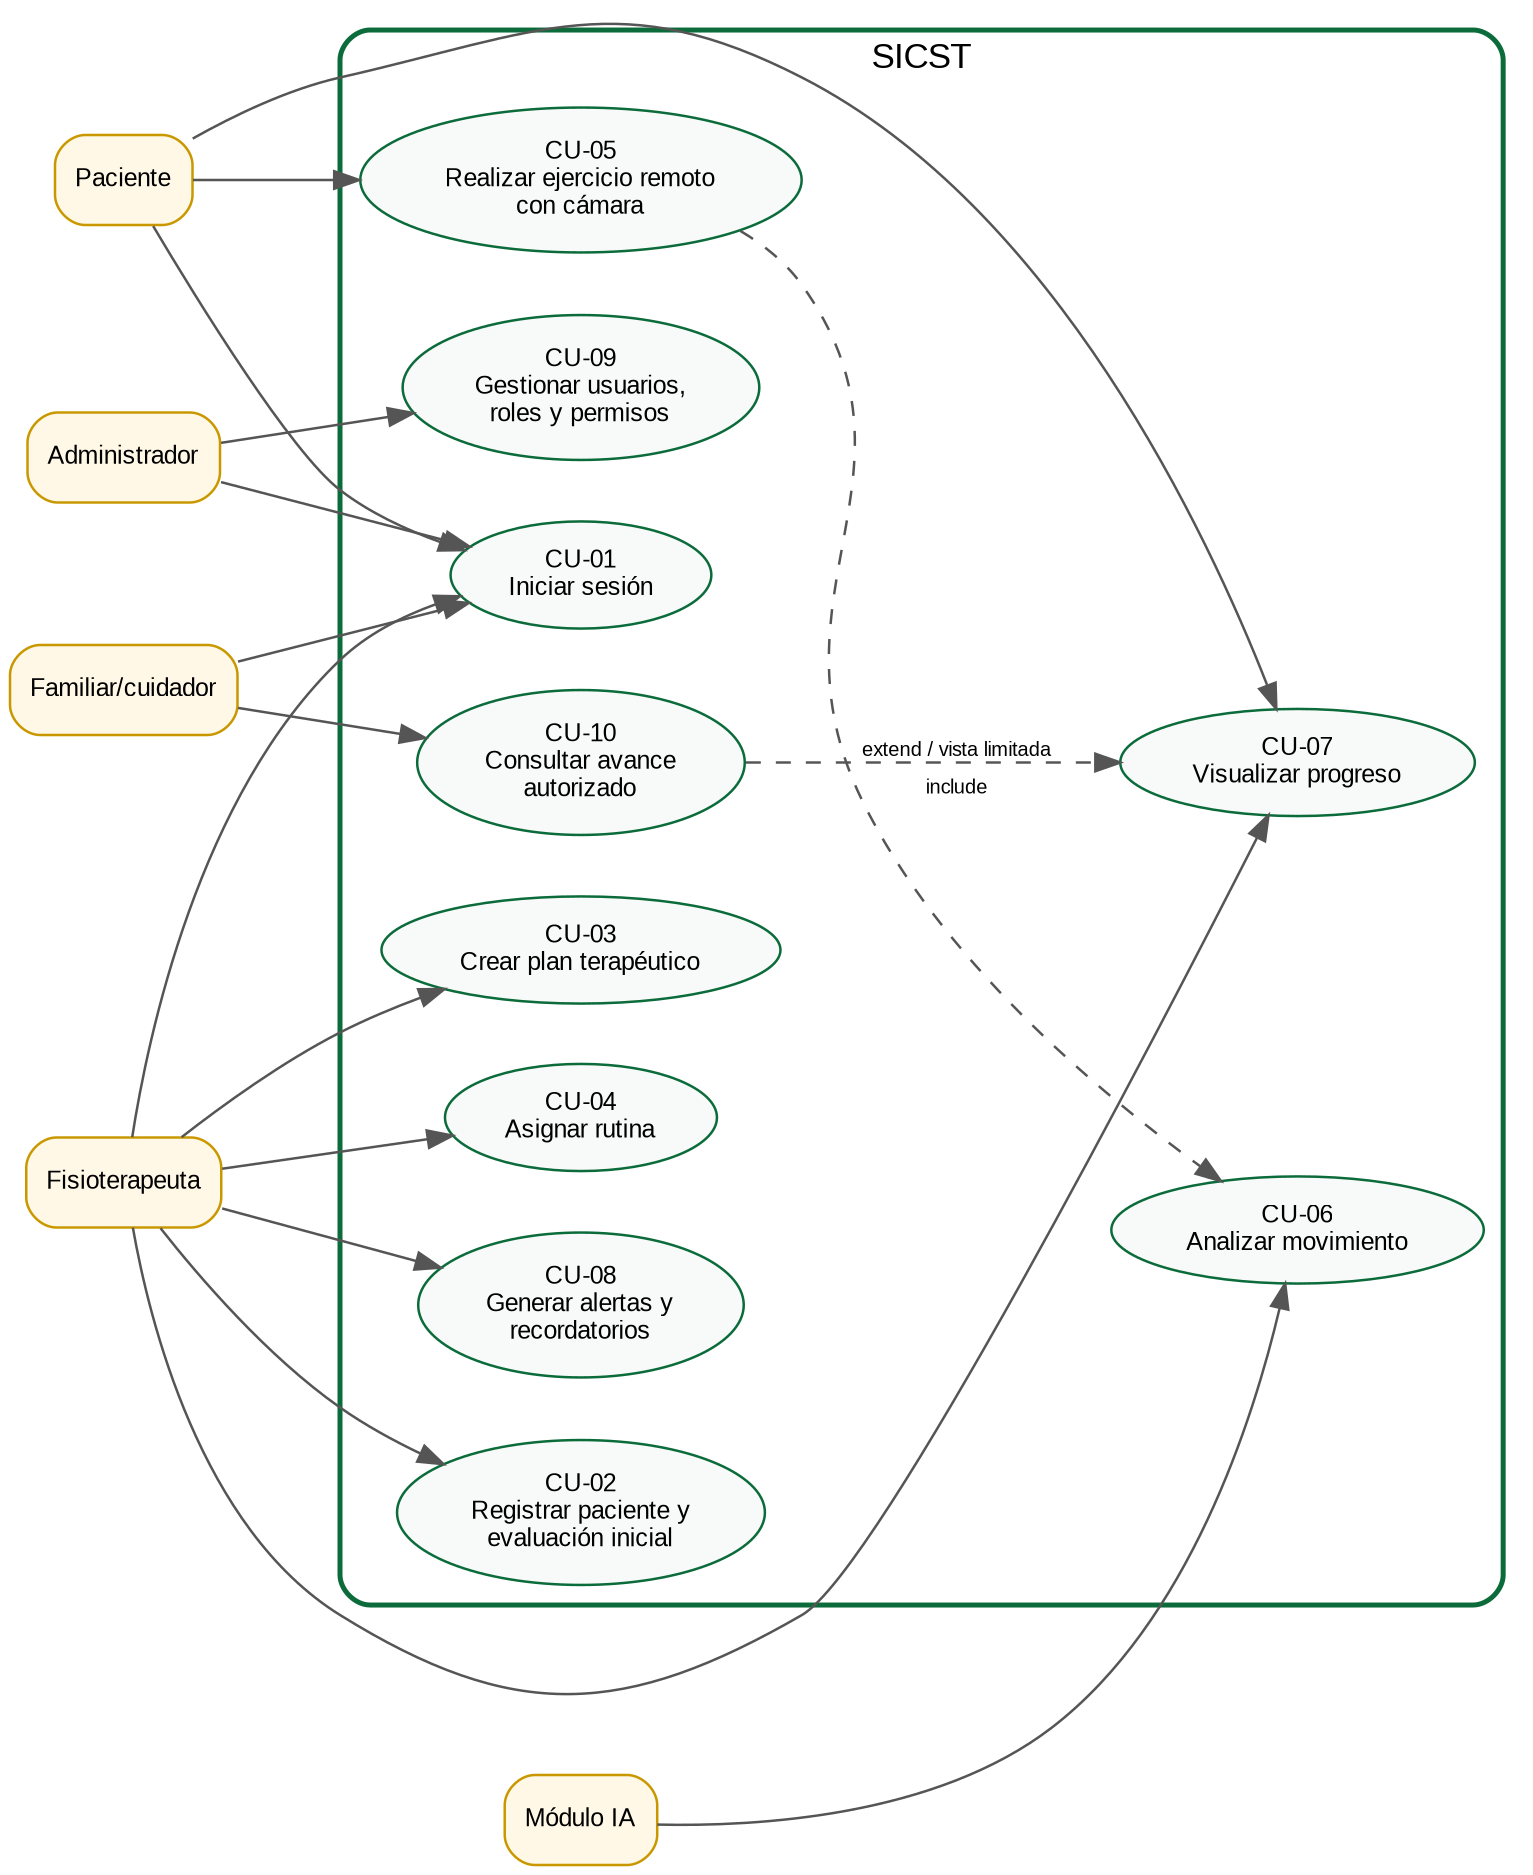
\includegraphics[width=0.82\textwidth]{figuras/casos_uso_10_pe5.png}\caption{Diagrama de casos de uso PE5 con diez casos.}\end{figure}

\small
\begin{longtable}{p{0.08\textwidth}p{0.24\textwidth}p{0.20\textwidth}p{0.20\textwidth}p{0.20\textwidth}}
\caption{Catálogo consolidado de casos de uso}\\
\toprule
\textbf{CU}&\textbf{Nombre}&\textbf{Actor principal}&\textbf{RF relacionados}&\textbf{Resultado observable}\\
\midrule\endfirsthead
\toprule
\textbf{CU}&\textbf{Nombre}&\textbf{Actor principal}&\textbf{RF relacionados}&\textbf{Resultado observable}\\
\midrule\endhead
CU-01 & Iniciar sesión & Usuario autorizado & RF-01, RF-02 & Acceso al panel correspondiente o rechazo de credenciales. \\
CU-02 & Registrar paciente y evaluación inicial & Fisioterapeuta & RF-03 a RF-14 & Ficha y evaluación inicial asociadas al paciente. \\
CU-03 & Crear plan terapéutico & Fisioterapeuta & RF-15, RF-16 & Plan terapéutico disponible para asignación de rutinas. \\
CU-04 & Asignar rutina terapéutica & Fisioterapeuta & RF-16, RF-17, RF-18, RF-31 & Rutina configurada y visible para el paciente. \\
CU-05 & Realizar ejercicio remoto con cámara & Paciente & RF-19 a RF-26 & Sesión remota registrada; la captura se habilita solo con consentimiento vigente. \\
CU-06 & Analizar movimiento & Paciente / módulo IA / fisioterapeuta & RF-21 a RF-25 & Análisis, repeticiones y retroalimentación asociados a la sesión. \\
CU-07 & Visualizar progreso terapéutico & Fisioterapeuta & RF-27, RF-30 & Indicadores de progreso y reportes consultables por periodo. \\
CU-08 & Generar alertas y recordatorios & Sistema / fisioterapeuta & RF-28, RF-29, RF-31, RF-33 & Alertas, recomendaciones y recordatorios registrados con estado y fecha. \\
CU-09 & Gestionar usuarios, roles y permisos & Administrador & RF-02 & Usuarios y permisos actualizados con control por rol. \\
CU-10 & Consultar avance autorizado & Familiar/cuidador autorizado & RF-32 & Resumen de avance limitado por autorización vigente. \\
\bottomrule\end{longtable}\normalsize

\subsection{DFD nivel 1}
Para completar la cadena de trazabilidad exigida se incorpora un DFD de nivel 1 con nueve procesos. P1 gestiona acceso/roles; P2 el registro clínico; P3 el plan; P4 rutinas; P5 sesión/captura; P6 análisis IA; P7 progreso/reportes; P8 alertas/recomendaciones/recordatorios; y P9 privacidad/acceso autorizado.

\begin{figure}[H]\centering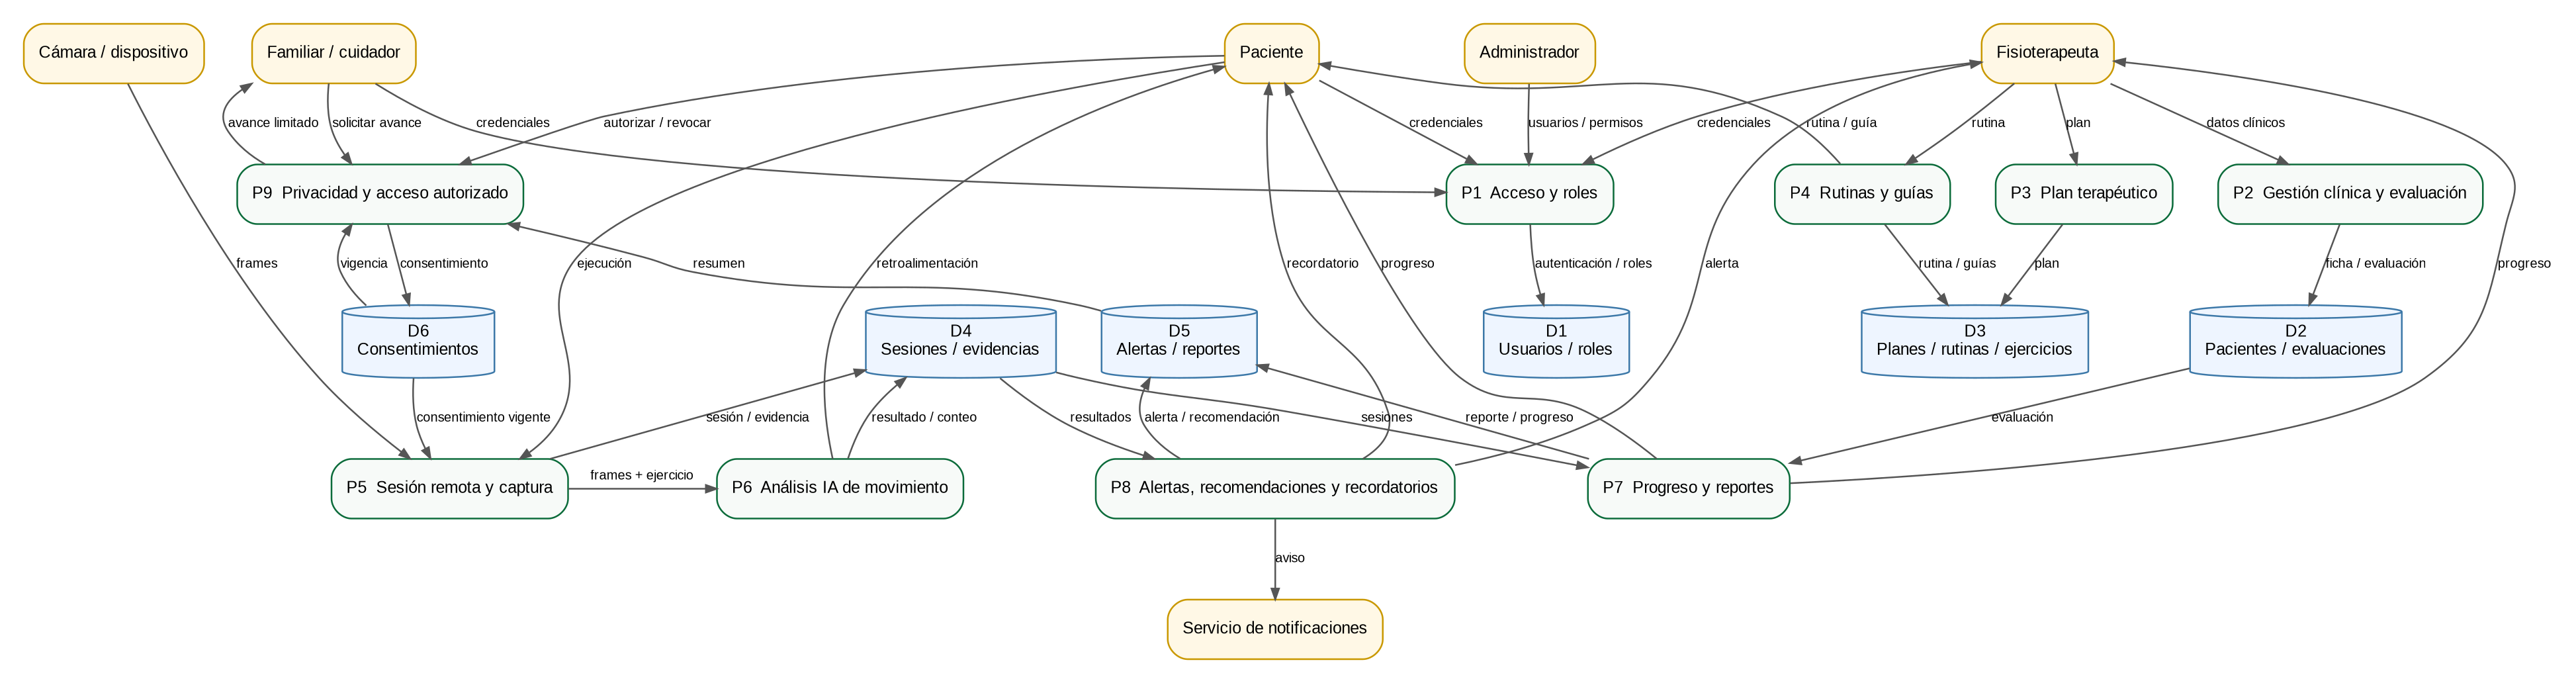
\includegraphics[width=\textwidth]{figuras/dfd_nivel1_pe5.png}\caption{DFD nivel 1 del SICST.}\end{figure}

\subsection{Clases y estados}
Las clases principales incluyen Usuario, Rol, Paciente, Fisioterapeuta, Administrador, FamiliarCuidador, EvaluacionInicial, SignosVitales, IndicadorClinico, PlanTerapeutico, Rutina, Ejercicio, EjercicioAsignado, SesionTerapia, EjecucionEjercicio, AnalisisMovimiento, Repeticion, Alerta, Recomendacion, Reporte, Notificacion, EvidenciaMultimedia y ConsentimientoInformado. La matriz traza cada requisito hacia las clases que realizan o almacenan su comportamiento.

\small
\begin{longtable}{p{0.23\textwidth}p{0.68\textwidth}}
\caption{Responsabilidades de las clases principales}\\
\toprule
\textbf{Clase}&\textbf{Responsabilidad en la trazabilidad y el dominio}\\
\midrule\endfirsthead
\toprule
\textbf{Clase}&\textbf{Responsabilidad en la trazabilidad y el dominio}\\
\midrule\endhead
Usuario & Representa a cualquier persona registrada en el sistema. Atributos de referencia: idUsuario, nombres, apellidos, correo, contraseña, estado. \\
Rol & Define permisos y restricciones de acceso. Atributos de referencia: idRol, nombreRol, permisos. \\
Paciente & Usuario que recibe tratamiento fisioterapéutico. Atributos de referencia: idPaciente, fechaNacimiento, contacto, diagnósticoReferencial. \\
Fisioterapeuta & Profesional encargado de evaluar, asignar rutinas y dar seguimiento. Atributos de referencia: idFisioterapeuta, especialidad, registroProfesional. \\
Administrador & Usuario encargado de gestionar cuentas, roles y parámetros. Atributos de referencia: idAdministrador, nivelAcceso. \\
FamiliarCuidador & Usuario autorizado para consultar avance limitado del paciente. Atributos de referencia: idFamiliar, parentesco, autorización. \\
EvaluacionInicial & Registro clínico inicial del paciente. Atributos de referencia: idEvaluacion, motivoConsulta, condiciónClinica, gravedad, fecha. \\
SignosVitales & Datos físicos registrados antes o durante la terapia. Atributos de referencia: idSignos, presiónArterial, frecuenciaCardiaca, observación. \\
IndicadorClinico & Valores como dolor, fatiga, rango de movimiento o capacidad funcional. Atributos de referencia: idIndicador, tipo, valor, escala, fecha. \\
PlanTerapeutico & Plan general de tratamiento asignado al paciente. Atributos de referencia: idPlan, objetivo, fechaInicio, fechaFin, estado. \\
Rutina & Conjunto de ejercicios definidos dentro del plan terapéutico. Atributos de referencia: idRutina, nombre, frecuencia, duraciónEstimada, estado. \\
Ejercicio & Ejercicio disponible en el catálogo del sistema. Atributos de referencia: idEjercicio, nombre, tipo, zonaCorporal, instrucciones. \\
EjercicioAsignado & Ejercicio configurado dentro de una rutina. Atributos de referencia: idAsignación, series, repeticiones, duración, observaciones. \\
SesionTerapia & Sesión realizada por el paciente. Atributos de referencia: idSesión, fechaHora, estado, modalidad. \\
EjecucionEjercicio & Registro de la ejecución de un ejercicio dentro de una sesión. Atributos de referencia: idEjecución, inicio, fin, repeticionesEsperadas, repeticionesValidas. \\
AnalisisMovimiento & Resultado del análisis realizado mediante cámara e IA. Atributos de referencia: idAnalisis, resultado, precisión, observaciónIA. \\
Repeticion & Registro individual de una repetición correcta o incorrecta. Atributos de referencia: idRepetición, número, estado, observación. \\
Alerta & Aviso generado por riesgo, error o incumplimiento, con estado Pendiente, Revisada o Atendida. Atributos de referencia: idAlerta, tipo, nivel, mensaje, fecha, estado, fechaRevision, fechaAtencion. \\
Recomendación & Sugerencia generada para el fisioterapeuta o paciente. Atributos de referencia: idRecomendacion, descripción, requiereValidación. \\
Reporte & Documento o resumen del progreso terapéutico. Atributos de referencia: idReporte, periodo, resumen, fechaGeneración. \\
Notificación & Mensaje enviado a paciente, fisioterapeuta o familiar autorizado. Atributos de referencia: idNotificacion, mensaje, destinatario, estado. \\
EvidenciaMultimedia & Imagen, video o audio relacionado con una sesión. Atributos de referencia: idEvidencia, tipo, url, fecha, consentimientoAsociado. \\
ConsentimientoInformado & Autorización del paciente para uso de datos y evidencias; su estado controla nuevas capturas y accesos asociados. Atributos de referencia: idConsentimiento, fecha, alcance, estado, fechaRevocatoria, firma. \\
\bottomrule\end{longtable}\normalsize

El diagrama de estados del tratamiento se complementa con estados de cuenta y consentimiento. Para tratamiento se mantienen estados como paciente registrado, evaluación completada, plan definido, rutina asignada, seguimiento, sesión en ejecución, progreso actualizado, alerta pendiente/revisada/atendida, ajuste, alta y suspensión. Para seguridad se usa Cuenta Activa/Inactiva/Bloqueada; para privacidad, Consentimiento Vigente/Revocado. Esto evita forzar un estado clínico a requisitos cuya semántica es de identidad o autorización.

\subsection{Componentes y despliegue}
La arquitectura lógica separa frontend, servicios de gestión clínica, rutinas, análisis IA, alertas/reportes, persistencia e integración con dispositivos. El despliegue académico debe declarar navegador, servidor/API, base de datos, dispositivo con cámara y dependencias necesarias. Los RNF de rendimiento no se consideran cumplidos hasta ejecutar las pruebas en un entorno de referencia documentado.

\section{Validación, inspección y evidencia empírica}
La fortaleza principal del proyecto está en la evidencia de campo. La línea base documenta entrevistas, consentimientos, fotografías, walkthrough, documentos de la organización y cuestionarios. Para PE5, la integración no debe reemplazar esos archivos por descripciones: cada afirmación debe conservar una ruta verificable en el repositorio.

\subsection{Inventario empírico vigente}
El ERS adjunto reporta 16 participantes/carpetas, 16 consentimientos, 15 entrevistas transcritas, 15 walkthrough con evidencia, 18 fotografías de campo, 15 fotografías de aplicación del cuestionario, 31 respuestas válidas y tres documentos originales de la organización. La duración acumulada de entrevistas se reporta en 124 minutos y 14 segundos. Tres walkthrough se identifican como mínimo formal: uno técnico con fisioterapeuta, uno no técnico con paciente y uno técnico en formación.

\begin{table}[H]\centering\caption{Distribución de las 31 respuestas válidas documentadas}\begin{tabular}{lrr}\toprule
\textbf{Perfil}&\textbf{Cantidad}&\textbf{Porcentaje}\\\midrule
Pacientes o expacientes&20&64.52\%\\
Familiares o cuidadores&8&25.81\%\\
Fisioterapeutas&3&9.68\%\\\midrule
Total&31&100\%\\\bottomrule
\end{tabular}\end{table}

El archivo bruto se conserva como evidencia de origen y el conjunto analítico de 31 registros se mantiene como la referencia cuantitativa del ERS/SRS final. La separación de ambos archivos evita alterar las respuestas originales y permite verificar qué conjunto se utilizó en las tablas de distribución, sin atribuir causas de exclusión que no estén documentadas.

\subsection{Fagan y CCB}
La inspección Fagan se documenta con Zambrano Moya Angelo Paul como Moderador y Lector, Contreras Chávez Kevin Germán como Inspector 1 y Morán Pilaguano Frixon Fernando como Inspector 2. Se revisaron 18 páginas efectivas y se consolidaron 16 defectos: 12 Mayores y 4 Menores, con densidad histórica de 0,89 defectos por página. Las correcciones armonizaron prioridades, trazabilidad, criterios verificables, alcance de IA y compatibilidad. Posteriormente, el CCB aprobó RF-33, RNF-13 y RES-15. La re-inspección PE5 contrasta D-01 a D-16 con el ERS final y registra los 16 defectos como cerrados, por lo que M6 = 0/58 = 0,000 defectos residuales por requisito.

\scriptsize
\begin{longtable}{p{0.08\textwidth}p{0.17\textwidth}p{0.11\textwidth}p{0.12\textwidth}p{0.42\textwidth}}
\caption{Re-inspección de los 16 defectos Fagan}\\
\toprule
\textbf{ID}&\textbf{Elemento}&\textbf{Severidad}&\textbf{Estado}&\textbf{Evidencia de cierre}\\
\midrule\endfirsthead
\toprule
\textbf{ID}&\textbf{Elemento}&\textbf{Severidad}&\textbf{Estado}&\textbf{Evidencia de cierre}\\
\midrule\endhead
D-01 & RF-28 & Mayor & Cerrado & Umbrales de alerta definidos: rutina vencida, EVA >= 7, Borg CR10 >= 7 y umbral configurado de repeticiones incorrectas. \\
D-02 & RNF-07 & Mayor & Cerrado & Disponibilidad definida por ventana de prueba declarada y cálculo reproducible. \\
D-03 & RF-15/RF-06/RF-07 & Mayor & Cerrado & RF-06 y RF-07 armonizados como Must respecto de RF-15. \\
D-04 & RNF-11 & Menor & Cerrado & Contraste mínimo 4,5:1 para texto normal. \\
D-05 & EV-*/EV2-* & Mayor & Cerrado & Correspondencia histórica de evidencias documentada. \\
D-06 & RNF-03 & Mayor & Cerrado & Entorno de referencia documentado para medir FPS. \\
D-07 & RF-19/RF-18 & Mayor & Cerrado & RF-18 armonizado como Must. \\
D-08 & EV-ENT-04 & Mayor & Cerrado & EV-ENT-04 eliminado como fuente independiente inconsistente. \\
D-09 & RNF-10 & Menor & Cerrado & Siete módulos principales enumerados y método de verificación definido. \\
D-10 & RNF-01 & Mayor & Cerrado & Muestra mínima de 10 usuarios: al menos 3 fisioterapeutas y 7 pacientes/expacientes. \\
D-11 & RF-24/RF-22 & Mayor & Cerrado & RF-22 armonizado como Must. \\
D-12 & RF-25 & Menor & Cerrado & Retroalimentación verificable con ejercicio, error detectado y acción/corrección sugerida. \\
D-13 & RF-22/RF-23/RF-24 & Mayor & Cerrado & Fuente armonizada a EV-ENT-03. \\
D-14 & RF-21 & Mayor & Cerrado & Análisis acotado a ejercicios compatibles y patrón configurado. \\
D-15 & RF-14 & Mayor & Cerrado & Relación armonizada con CU-02. \\
D-16 & RNF-09 & Menor & Cerrado & Compatibilidad alineada con Chrome, Edge y Firefox. \\
\bottomrule\end{longtable}\normalsize

\subsection{Ejecución controlada del protocolo de explicabilidad}
El protocolo se ejercitó mediante una simulación controlada con datos sintéticos, separada de la evidencia humana real. Se estructuraron dos rondas de seis perfiles cada una, combinando fisioterapeuta, estudiante de fisioterapia y usuario no técnico. El instrumento empleó Q01--Q11 en escala Likert de 1 a 5 y Q12 como comentario abierto. Entre rondas se refinó la explicación para destacar causa, evidencia y acción segura sugerida.


\begin{table}[H]\centering\caption{Instrumento Q01--Q12 de la ejecución controlada}
\small
\begin{tabularx}{\textwidth}{p{0.08\textwidth}p{0.25\textwidth}X}
\toprule
\textbf{Ítem}&\textbf{Dimensión}&\textbf{Criterio evaluado}\\\midrule
Q01&Necesidad&La explicación aporta información necesaria para comprender la salida del sistema.\\
Q02&Claridad&El mensaje se entiende sin conocimientos técnicos adicionales.\\
Q03&Relevancia&La explicación se concentra en información útil para la situación presentada.\\
Q04&Detalle&El nivel de detalle es suficiente sin sobrecargar al usuario.\\
Q05&Temporalidad&La explicación aparece en el momento adecuado del flujo.\\
Q06&Evidencia&El mensaje identifica el dato, señal o evento que sustenta la salida.\\
Q07&Comprensión&El usuario puede explicar con sus palabras qué ocurrió y por qué.\\
Q08&Acción&La salida indica una acción segura o un siguiente paso comprensible.\\
Q09&Confianza calibrada&El mensaje comunica límites y evita presentar la salida como certeza clínica.\\
Q10&Control/revisión&El usuario identifica cómo revisar, confirmar o escalar la recomendación.\\
Q11&Satisfacción&Valoración global de la explicación presentada.\\
Q12&Comentario abierto&Observación cualitativa sobre cambios necesarios en la explicación.\\
\bottomrule
\end{tabularx}
\normalsize
\end{table}

La ejecución controlada utiliza códigos SIM-R1-01 a SIM-R1-06 y SIM-R2-01 a SIM-R2-06. Los perfiles representan combinaciones plausibles de usuario técnico y no técnico únicamente para ejercitar el protocolo; no corresponden a personas identificables ni se mezclan con la evidencia de campo. El análisis reproduce las medias desde los CSV y conserva el script que calcula los indicadores, de forma que los resultados de la simulación pueden ser verificados sin edición manual.


\begin{table}[H]\centering\caption{Resultados de la simulación controlada de explicabilidad}
\begin{tabular}{lccc}\toprule
\textbf{Indicador}&\textbf{Ronda 1}&\textbf{Ronda 2}&\textbf{Variación}\\\midrule
N.° de perfiles&6&6&--\\
Media global Q01--Q11&3,58&4,65&+1,08\\
Claridad (Q02)&3,67&4,67&+1,00\\
Comprensión (Q07)&3,33&4,67&+1,34\\
Control/revisión (Q10)&2,83&4,33&+1,50\\
Satisfacción (Q11)&3,67&4,83&+1,16\\\bottomrule
\end{tabular}\end{table}

Los comentarios de la primera ronda se orientaron a reducir extensión, hacer visible la causa y separar la recomendación práctica. La segunda ronda mostró mejores puntuaciones en claridad, comprensión, control y satisfacción. Los archivos CSV y el script de análisis se conservan como evidencia reproducible del ejercicio controlado.


\subsection{Validez, alcance y limitaciones de la evidencia}
La evidencia se interpreta según su naturaleza y propósito. Las entrevistas, consentimientos, cuestionarios, documentos y walkthrough pertenecen al trabajo de campo del proyecto y sustentan necesidades, restricciones y validaciones documentales. La ejecución Q01--Q12, en cambio, es una simulación controlada destinada a ejercitar el protocolo de explicabilidad y su análisis reproducible; sus resultados no se generalizan a una población clínica ni sustituyen una validación con usuarios reales.

\begin{table}[H]\centering\caption{Amenazas de validez y controles aplicados}
\small
\begin{tabularx}{\textwidth}{p{0.20\textwidth}p{0.31\textwidth}X}
\toprule
\textbf{Dimensión}&\textbf{Riesgo}&\textbf{Control aplicado}\\\midrule
Validez de constructo&Confundir una necesidad expresada por usuarios con una función ya implementada.&Se mantiene separación entre evidencia de elicitación, requisito especificado, criterio de aceptación y estado del MVP.\\
Validez interna&Mezclar versiones históricas de evidencias o identificadores distintos.&La línea base PE5 conserva códigos de fuente y la matriz final solo utiliza identificadores definidos en el ERS/SRS final.\\
Validez externa&Generalizar resultados de una práctica académica a pacientes o entornos clínicos reales.&El alcance se limita al prototipo académico; no se declaran eficacia clínica, diagnóstico, certificación médica ni generalización poblacional.\\
Validez de conclusión&Interpretar los resultados de la simulación de explicabilidad como evidencia empírica humana.&Los archivos SIM-R1/SIM-R2 se almacenan separados, se identifican como simulación controlada y se usan únicamente para comprobar el procedimiento de análisis.\\
Trazabilidad de evidencia&Perder la relación entre una conclusión y el artefacto que la respalda.&Las afirmaciones de calidad documental se anclan en RF/RNF, matriz, BDD, CP, Fagan, CCB y archivos de métricas.\\
\bottomrule
\end{tabularx}
\normalsize
\end{table}

Estas limitaciones no invalidan el cierre de Ingeniería de Requisitos: delimitan qué afirmaciones son documentales, cuáles proceden de trabajo de campo y cuáles corresponden a una práctica controlada. El criterio de aceptación del PE5 es la coherencia y auditabilidad de la especificación, no demostrar efectividad terapéutica del software.

\section{Gestión y trazabilidad end-to-end}
La trazabilidad final se reconstruye con la cadena principal exigida por la rúbrica: Fuente $\rightarrow$ Requisito $\rightarrow$ Caso de uso $\rightarrow$ Clase UML $\rightarrow$ Estado $\rightarrow$ BDD $\rightarrow$ Caso de prueba. Como campos complementarios se conservan Proceso DFD, Historia de usuario, Prioridad y Estado de la traza. Para RF también se enlaza una HU real. Los RNF usan N/A justificado en Historia de usuario, en vez de crear identificadores que no existen.

\subsection{Backlog completo}
La tabla siguiente muestra las 33 historias y su BDD principal. El archivo CSV conserva además el caso de prueba conceptual y la fuente.
\scriptsize
\begin{longtable}{p{0.06\textwidth}p{0.06\textwidth}p{0.37\textwidth}p{0.41\textwidth}}
\caption{Historias de usuario y BDD del SICST}\\\toprule
\textbf{HU}&\textbf{RF}&\textbf{Historia}&\textbf{BDD}\\\midrule\endfirsthead
\toprule\textbf{HU}&\textbf{RF}&\textbf{Historia}&\textbf{BDD}\\\midrule\endhead

HU-01 & RF-01 & Como usuario autorizado, quiero autenticar usuarios, para acceder únicamente a las funciones permitidas por mi rol. & Dado un usuario registrado y activo con un rol asignado; cuando ingresa credenciales válidas; entonces el sistema autentica al usuario, carga el panel de su rol y bloquea funciones no autorizadas \\
HU-02 & RF-02 & Como administrador, quiero gestionar roles y permisos, para controlar quién puede acceder a cada función y dato sensible. & Dado un administrador autenticado; cuando crea o modifica un usuario y asigna un rol; entonces el sistema guarda el cambio y aplica los permisos definidos para ese rol \\
HU-03 & RF-03 & Como fisioterapeuta, quiero registrar datos generales del paciente, para disponer de una ficha identificable y completa del paciente. & Dado un fisioterapeuta autenticado; cuando registra los datos obligatorios de un paciente; entonces el sistema crea la ficha del paciente y permite consultarla \\
HU-04 & RF-04 & Como fisioterapeuta, quiero registrar motivo de consulta, para documentar la razón clínica que origina la terapia. & Dado un paciente registrado; cuando el fisioterapeuta registra el motivo de consulta; entonces el sistema lo asocia al paciente y lo muestra en la evaluación inicial \\
HU-05 & RF-05 & Como fisioterapeuta, quiero registrar antecedentes terapeuticos, para considerar lesiones y tratamientos previos al planificar la rehabilitación. & Dado un paciente registrado; cuando el fisioterapeuta registra o actualiza antecedentes terapéuticos; entonces el sistema los conserva en la ficha del paciente \\
HU-06 & RF-06 & Como fisioterapeuta, quiero clasificar condición clínica, para organizar el seguimiento según la condición clínica registrada. & Dado un paciente con evaluación inicial; cuando el fisioterapeuta selecciona la condición clínica; entonces el sistema guarda la clasificación asociada al paciente \\
HU-07 & RF-07 & Como fisioterapeuta, quiero clasificar nivel de gravedad, para ajustar la intensidad y el seguimiento al nivel de gravedad. & Dado un paciente con condición clínica registrada; cuando el fisioterapeuta clasifica la gravedad; entonces el sistema guarda el nivel como leve, moderado o grave y lo vincula al plan terapéutico \\
HU-08 & RF-08 & Como fisioterapeuta, quiero registrar signos vitales, para comprobar el estado fisiológico antes y durante la terapia. & Dado un paciente en evaluación; cuando el fisioterapeuta registra signos vitales; entonces el sistema guarda valores, fecha, hora y responsable y los muestra en la evaluación \\
HU-09 & RF-09 & Como fisioterapeuta, quiero registrar rangos de movimiento, para comparar la movilidad del paciente a lo largo del tratamiento. & Dado un paciente en evaluación; cuando el fisioterapeuta registra el rango de movimiento de una articulación; entonces el sistema guarda la medición con unidad y la asocia al paciente \\
HU-10 & RF-10 & Como fisioterapeuta, quiero registrar pruebas terapéuticas, para conservar resultados de pruebas terapéuticas para la evaluación. & Dado un paciente en evaluación; cuando el fisioterapeuta registra una prueba terapéutica y su resultado; entonces el sistema conserva el resultado y permite consultarlo posteriormente \\
HU-11 & RF-11 & Como paciente o fisioterapeuta, quiero registrar nivel de dolor, para seguir la evolución del dolor y detectar cambios relevantes. & Dado un paciente o fisioterapeuta autorizado; cuando registra un nivel de dolor en la escala definida; entonces el sistema guarda el valor con fecha y sesión y lo incorpora al historial de progreso \\
HU-12 & RF-12 & Como paciente o fisioterapeuta, quiero registrar nivel de fatiga, para seguir la fatiga y evitar sobrecarga durante la rehabilitación. & Dado un paciente o fisioterapeuta autorizado; cuando registra el nivel de fatiga en la escala definida; entonces el sistema guarda el valor por sesión y lo relaciona con dolor y cumplimiento \\
HU-13 & RF-13 & Como fisioterapeuta, quiero registrar capacidad funcional, para comparar el desempeño funcional entre evaluaciones. & Dado un paciente en evaluación; cuando el fisioterapeuta registra la capacidad funcional; entonces el sistema guarda el indicador y lo hace disponible en historial y reportes \\
HU-14 & RF-14 & Como fisioterapeuta, quiero registrar observaciones por sesión, para mantener contexto clínico de lo ocurrido en cada sesión. & Dada una sesión terapéutica identificada; cuando el fisioterapeuta registra una observación; entonces el sistema la guarda asociada a la sesión, paciente, fecha y responsable \\
HU-15 & RF-15 & Como fisioterapeuta, quiero crear plan terapéutico personalizado, para organizar objetivos y acciones terapéuticas por paciente. & Dado un paciente con evaluación inicial suficiente; cuando el fisioterapeuta crea un plan terapéutico; entonces el sistema guarda el plan asociado al paciente y lo deja disponible para asignar rutinas \\
HU-16 & RF-16 & Como fisioterapeuta, quiero gestionar catálogo de ejercicios, para reutilizar ejercicios definidos con información consistente. & Dado un fisioterapeuta autenticado; cuando registra o actualiza un ejercicio con sus campos obligatorios; entonces el sistema guarda el ejercicio en el catálogo con tipo, zona corporal, descripción e instrucciones \\
HU-17 & RF-17 & Como fisioterapeuta, quiero asignar rutina terapéutica, para entregar al paciente una rutina concreta y personalizada. & Dado un plan terapéutico activo y ejercicios disponibles; cuando el fisioterapeuta selecciona ejercicios, series, repeticiones, duración y frecuencia; entonces el sistema crea la rutina y la muestra en el panel del paciente \\
HU-18 & RF-18 & Como paciente, quiero mostrar guías visuales, para ejecutar los ejercicios con instrucciones visuales comprensibles. & Dada una rutina asignada; cuando el paciente consulta un ejercicio; entonces el sistema muestra instrucciones y el recurso visual disponible antes de iniciar la ejecución \\
HU-19 & RF-19 & Como paciente, quiero iniciar sesión remota de ejercicios, para realizar la rutina asignada desde casa y registrar la sesión. & Dada una rutina pendiente asignada al paciente; cuando el paciente inicia la ejecución remota; entonces el sistema crea una sesión vinculada a la rutina y registra fecha y hora de inicio \\
HU-20 & RF-20 & Como paciente, quiero capturar movimiento con cámara, para habilitar el análisis de movimiento únicamente cuando lo autorice. & Dada una sesión remota que requiere cámara; cuando el paciente revisa la finalidad y otorga consentimiento vigente; entonces el sistema habilita la captura; si rechaza o revoca, no captura y ofrece la alternativa sin cámara \\
HU-21 & RF-21 & Como fisioterapeuta, quiero analizar movimiento del paciente, para obtener una evaluación automática de la ejecución compatible con IA. & Dado un ejercicio compatible con análisis automático, un patrón configurado y una sesión con captura válida; cuando el módulo IA recibe los frames; entonces el sistema genera un resultado de análisis asociado a la sesión y al ejercicio \\
HU-22 & RF-22 & Como fisioterapeuta, quiero detectar errores de postura, para identificar desviaciones posturales durante el ejercicio. & Dado un análisis de movimiento activo; cuando el patrón observado se desvía del rango configurado; entonces el sistema registra el error postural y lo vincula al instante o repetición correspondiente \\
HU-23 & RF-23 & Como paciente, quiero contar repeticiones correctas, para conocer cuántas repeticiones se realizaron correctamente. & Dado un ejercicio compatible y una secuencia de movimiento analizada; cuando una repetición cumple el patrón configurado; entonces el sistema incrementa el conteo de repeticiones correctas y conserva el resultado \\
HU-24 & RF-24 & Como paciente, quiero rechazar repeticiones incorrectas, para evitar que repeticiones técnicamente incorrectas se contabilicen como válidas. & Dada una repetición analizada que incumple el patrón configurado; cuando el módulo IA la clasifica como incorrecta; entonces el sistema no la suma al conteo válido y registra la causa de rechazo \\
HU-25 & RF-25 & Como paciente, quiero generar retroalimentación automática, para recibir una corrección comprensible durante la ejecución. & Dado un error postural o una repetición incorrecta detectada durante una sesión; cuando el sistema genera retroalimentación; entonces muestra al paciente una explicación breve con ejercicio, error detectado y acción segura recomendada \\
HU-26 & RF-26 & Como fisioterapeuta, quiero registrar evidencia de cumplimiento, para dejar evidencia verificable del cumplimiento de la rutina. & Dada una sesión finalizada o un hito de cumplimiento; cuando el sistema guarda el resultado de la rutina; entonces registra evidencia con paciente, sesión, fecha, hora y resultado de cumplimiento \\
HU-27 & RF-27 & Como fisioterapeuta, quiero visualizar progreso terapéutico, para comparar la evolución del paciente mediante indicadores organizados. & Dado un paciente con sesiones o evaluaciones previas; cuando el fisioterapeuta consulta su progreso; entonces el sistema presenta indicadores organizados por fecha y sesión respetando el rol del usuario \\
HU-28 & RF-28 & Como fisioterapeuta, quiero generar alertas terapéuticas, para atender oportunamente situaciones que requieren seguimiento. & Dada una sesión que cumple una regla de alerta configurada; cuando se guarda el resultado de la sesión; entonces el sistema crea una alerta con paciente, causa, fecha, hora y estado Pendiente y la muestra al fisioterapeuta \\
HU-29 & RF-29 & Como fisioterapeuta, quiero generar recomendaciones de seguimiento, para contar con apoyo para decidir el siguiente paso de seguimiento sin sustituir mi criterio profesional. & Dado un paciente con información de seguimiento disponible; cuando el sistema genera una recomendación; entonces la muestra como apoyo, explica sus factores principales e indica que requiere validación profesional \\
HU-30 & RF-30 & Como fisioterapeuta, quiero generar reportes del tratamiento, para resumir y comunicar la evolución terapéutica por periodo. & Dado un paciente con historial terapéutico; cuando el fisioterapeuta selecciona un periodo y solicita un reporte; entonces el sistema genera un reporte con indicadores, rutinas, cumplimiento, dolor, fatiga y observaciones y permite exportarlo \\
HU-31 & RF-31 & Como paciente, quiero enviar recordatorios automáticos, para recordar las rutinas pendientes y mejorar la adherencia. & Dada una rutina pendiente con frecuencia y horario definidos; cuando llega el momento programado sin registro de cumplimiento; entonces el sistema envía un recordatorio al paciente y registra el intento de notificación \\
HU-32 & RF-32 & Como familiar o cuidador autorizado, quiero consultar avance autorizado, para consultar únicamente el avance que el paciente me haya autorizado. & Dado un familiar o cuidador autenticado y una autorización vigente del paciente; cuando solicita consultar el avance; entonces el sistema muestra únicamente el resumen autorizado; si la autorización no existe o fue revocada, deniega el acceso \\
HU-33 & RF-33 & Como fisioterapeuta, quiero gestionar estado y escalamiento de alertas terapéuticas, para distinguir alertas pendientes, revisadas y atendidas y mantener su trazabilidad. & Dada una alerta en estado Pendiente; cuando el fisioterapeuta la revisa o atiende; entonces el sistema actualiza el estado a Revisada o Atendida y conserva la fecha, hora y responsable del cambio \\
\bottomrule\end{longtable}\normalsize

\subsection{Matriz final}
La matriz final adopta exactamente la cadena requerida por la rúbrica: Fuente $\rightarrow$ RF/RNF $\rightarrow$ CU $\rightarrow$ Clase UML $\rightarrow$ Estado $\rightarrow$ BDD $\rightarrow$ Caso de prueba. Como campos complementarios conserva Proceso DFD, Historia de usuario, Prioridad y Estado de la traza. La versión completa contiene 58 filas: 33 RF, 15 RNF generales y 10 RNF específicos de IA; se reproduce íntegramente en el Anexo B y se mantiene en CSV para auditoría.

\begin{table}[H]\centering\caption{Cobertura de la matriz de trazabilidad final}
\begin{tabular}{lrrl}\toprule
\textbf{Elemento}&\textbf{Total}&\textbf{Trazado}&\textbf{Cobertura}\\\midrule
RF&33&33&100 \%\\
RNF generales&15&15&100 \%\\
RNF específicos de IA&10&10&100 \%\\
Historias HU vinculadas a RF&33&33&100 \%\\\bottomrule
\end{tabular}\end{table}

\setlength{\tabcolsep}{2.5pt}
\scriptsize
\begin{longtable}{p{0.09\textwidth}p{0.15\textwidth}p{0.08\textwidth}p{0.22\textwidth}p{0.17\textwidth}p{0.14\textwidth}p{0.07\textwidth}p{0.08\textwidth}}
\caption{Muestra auditada de trazas representativas}\\
\toprule
\textbf{Req.}&\textbf{Fuente}&\textbf{CU}&\textbf{Clase UML}&\textbf{Estado}&\textbf{BDD / CP}&\textbf{DFD}&\textbf{HU}\\
\midrule\endfirsthead
\toprule
\textbf{Req.}&\textbf{Fuente}&\textbf{CU}&\textbf{Clase UML}&\textbf{Estado}&\textbf{BDD / CP}&\textbf{DFD}&\textbf{HU}\\
\midrule\endhead
RF-01 & EV-CUE-01 & CU-01 & Usuario; Rol & Cuenta: Activa / Inactiva / Bloqueada & BDD-01 / CP-01 & P1 & HU-01 \\
RF-02 & EV-CUE-01 & CU-09 & Administrador; Usuario; Rol & Cuenta: Activa / Inactiva / Bloqueada & BDD-02 / CP-02 & P1 & HU-02 \\
RF-17 & EV-ENT-01, EV-ENT-02 & CU-04 & Fisioterapeuta; Paciente; Rutina; EjercicioAsignado; Ejercicio; Notificacion & Rutina asignada & BDD-17 / CP-17 & P4 & HU-17 \\
RF-20 & EV-ENT-03, EV-CONS-01 & CU-05 & Paciente; SesionTerapia; EjecucionEjercicio; EvidenciaMultimedia; ConsentimientoInformado & En seguimiento / Sesion en ejecucion / Progreso actualizado & BDD-20 / CP-20 & P5 & HU-20 \\
RF-21 & EV-ENT-03 & CU-06 & AnalisisMovimiento; Repeticion; Alerta; Recomendacion & Sesion en ejecucion / Progreso actualizado & BDD-21 / CP-21 & P6 & HU-21 \\
RF-28 & EV-ENT-03 & CU-08 & Alerta; Recomendacion; Notificacion; SesionTerapia; Fisioterapeuta & Alerta pendiente / Revisada / Atendida & BDD-28 / CP-28 & P8 & HU-28 \\
RF-32 & EV-CONS-01 & CU-10 & FamiliarCuidador; Paciente; ConsentimientoInformado; Reporte & Consentimiento: Vigente / Revocado & BDD-32 / CP-32 & P9 & HU-32 \\
RF-33 & RFC-01 / CCB PE4 & CU-08 & Alerta; Recomendacion; Notificacion; SesionTerapia; Fisioterapeuta & Alerta pendiente / Revisada / Atendida & BDD-33 / CP-33 & P8 & HU-33 \\
RNF-06 & LOPDP; EV-CONS-01 & CU-01 / CU-09 / CU-10 & Usuario; Rol; ConsentimientoInformado; Reporte & Cuenta activa / Consentimiento vigente & BDD-RNF-06 / CP-RNF-06 & P1 / P9 & N/A \\
RNF-12 & LOPDP; EV-CONS-01; RES-02/RES-15 & CU-05 / CU-10 & ConsentimientoInformado; EvidenciaMultimedia; FamiliarCuidador & Consentimiento vigente / revocado & BDD-RNF-12 / CP-RNF-12 & P5 / P9 & N/A \\
RNF-IA1-XAI01 & RNF-XAI-01 del ERS; PE5 C3 & CU-06 & AnalisisMovimiento; Recomendacion & Sesion en ejecucion & BDD-RNF-IA1-XAI01 / CP-RNF-IA1-XAI01 & P6 & N/A \\
RNF-IA2-XAI01 & PE5 C3; RF-28/RF-29; RES-01/RES-03 & CU-08 & Alerta; Recomendacion & Alerta pendiente & BDD-RNF-IA2-XAI01 / CP-RNF-IA2-XAI01 & P8 & N/A \\
\bottomrule\end{longtable}\normalsize\setlength{\tabcolsep}{6pt}

\subsection{Huérfanos, cadenas rotas y sincronización}
La auditoría final no registra requisitos huérfanos ni cadenas rotas. Los 33 RF tienen fuente identificada, CU, clase UML, proceso DFD, estado, BDD y caso de prueba; los 33 RF también disponen de HU. Para RNF y RNF-IA se usa N/A únicamente en Historia de usuario cuando la calidad es transversal, sin crear historias ficticias. La sincronización backlog $\leftrightarrow$ ERS queda en 33/33 RF y la trazabilidad M4 se audita sobre los 33 RF, tal como establece la rúbrica.

\section{Requisitos de inteligencia artificial}
PE5 exige al menos dos componentes de IA plausibles para el dominio, con requisitos de rendimiento, equidad y explicabilidad medibles. La especificación evita duplicar RF: reutiliza obligaciones funcionales existentes y agrega RNF específicos solo donde hace falta expresar propiedades del modelo.


\begin{table}[H]\centering\caption{Cinco bloques de especificación de los componentes de IA}
\small
\begin{tabularx}{\textwidth}{p{0.17\textwidth}X X}
\toprule
\textbf{Bloque}&\textbf{IA-01: análisis de movimiento}&\textbf{IA-02: priorización de alertas y recomendaciones}\\\midrule
Función, entradas y salidas&Entradas: frames autorizados, ejercicio esperado y patrón configurado. Salidas: análisis de ejecución, repeticiones, desviación detectada y retroalimentación explicable.&Entradas: dolor, fatiga, cumplimiento, progreso, errores y reglas de seguimiento. Salidas: prioridad, alerta/recomendación, factores principales y estado para revisión.\\
Datos y privacidad&Consentimiento previo, minimización de datos, condiciones de captura, versión del conjunto y exclusión de información identificable del dataset público.&Uso de indicadores ya registrados, control por rol, trazabilidad del criterio experto y protección de datos clínicos.\\
Rendimiento y equidad&15 FPS como RNF general, precisión de conteo $\geq85$ \%, latencia p95 $\leq2$ s y brechas F1/recall $\leq0,05$ entre grupos definidos.&Precision y recall $\geq0,80$, latencia p95 $\leq1$ s y brechas TPR/FPR $\leq0,05$ entre grupos definidos.\\
Explicabilidad y control humano&Explicación de causa, evidencia y acción segura en $\leq60$ palabras; claridad media $\geq4/5$; fisioterapeuta puede revisar la salida.&Hasta tres factores principales, advertencia no diagnóstica y acción sugerida; claridad media $\geq4/5$; ninguna recomendación modifica tratamiento automáticamente.\\
Riesgo, fallback y monitoreo&Sin consentimiento o captura suficiente se desactiva el análisis y permanece disponible la rutina sin cámara. Se monitorizan latencia, precisión y brechas por versión.&Si no existen datos suficientes o el indicador supera límites de operación, se muestra estado no concluyente y se deriva a revisión profesional. Se monitorizan precisión, recall, falsas alertas y brechas.\\
\bottomrule
\end{tabularx}
\normalsize
\end{table}


\subsection{IA-01: análisis de movimiento por visión por computadora}
IA-01 recibe frames de una sesión autorizada, identifica el ejercicio esperado y evalúa el patrón de movimiento. Sus RF mínimos son RF-21, RF-22 y RF-23; RF-24 y RF-25 complementan rechazo y retroalimentación. RNF-03 exige al menos 15 FPS y RNF-04 una precisión de conteo mínima de 85\%. Se agrega latencia p95, dos controles de equidad y un requisito de explicabilidad. Técnicas de estimación de pose y pipelines de percepción son pertinentes al dominio de rehabilitación asistida por visión \cite{cao2021,lugaresi2019,zheng2022}.

El modo degradado es obligatorio: sin consentimiento vigente, cámara suficiente, iluminación adecuada o patrón configurado, el sistema no debe inventar un análisis; mantiene acceso a la rutina/guía y comunica la limitación. La salida es de apoyo y no sustituye evaluación profesional.

\subsection{IA-02: priorización de alertas y recomendaciones}
IA-02 procesa indicadores ya registrados —dolor, fatiga, cumplimiento, errores y progreso— para apoyar la priorización del seguimiento. Se apoya en RF-25, RF-28 y RF-29; RF-33 conserva el estado y la revisión humana. El componente nunca decide diagnóstico ni tratamiento. La salida explica factores de activación y mantiene una advertencia no diagnóstica.

\subsection{RNF específicos de IA}
\small
\begin{longtable}{p{0.14\textwidth}p{0.22\textwidth}p{0.12\textwidth}p{0.42\textwidth}}
\caption{RNF específicos de IA para PE5}\\\toprule
\textbf{ID}&\textbf{Componente}&\textbf{Tipo}&\textbf{Umbral y método}\\\midrule\endfirsthead
\toprule\textbf{ID}&\textbf{Componente}&\textbf{Tipo}&\textbf{Umbral y método}\\\midrule\endhead

RNF-IA1-P01 & IA-01 Visión por computadora & Rendimiento & Latencia extremo a extremo p95 ≤ 2 s desde recepción del frame evaluable hasta presentación de retroalimentación. 100 eventos cronometrados en equipo de referencia; calcular p95. \\
RNF-IA1-EQ01 & IA-01 Visión por computadora & Equidad & Brecha absoluta de F1 entre grupos 18-39 y ≥40 años ≤ 0.05, siempre que cada grupo disponga de muestra mínima documentada. Conjunto de evaluación estratificado; bootstrap 95 \% y reporte por grupo. \\
RNF-IA1-EQ02 & IA-01 Visión por computadora & Equidad & Brecha absoluta de recall entre grupos de limitación leve y moderada ≤ 0.05, con tamaño de muestra mínimo documentado. Evaluación estratificada y reporte de recall e intervalo por grupo. \\
RNF-IA1-XAI01 & IA-01 Visión por computadora & Explicabilidad & Explicación ≤ 60 palabras, mostrada ≤ 2 s, con claridad media ≥ 4/5 y presencia de causa, evidencia y acción. Prueba cronometrada + cuestionario de comprensión con usuarios. \\
RNF-IA2-P01 & IA-02 Priorización de alertas y recomendaciones & Rendimiento & Precision ≥ 0.80 para la clase “requiere seguimiento prioritario”. Conjunto de evaluación etiquetado por al menos un fisioterapeuta responsable; matriz de confusión. \\
RNF-IA2-P02 & IA-02 Priorización de alertas y recomendaciones & Rendimiento & Recall ≥ 0.80 para la clase “requiere seguimiento prioritario”. Mismo conjunto de evaluación etiquetado; matriz de confusión. \\
RNF-IA2-P03 & IA-02 Priorización de alertas y recomendaciones & Rendimiento & Latencia p95 ≤ 1 s por evento en entorno de prueba documentado. 100 eventos cronometrados; calcular p95. \\
RNF-IA2-EQ01 & IA-02 Priorización de alertas y recomendaciones & Equidad & Brecha absoluta de TPR entre grupos 18-39 y ≥40 años ≤ 0.05, con tamaño mínimo documentado. Evaluación estratificada; TPR e intervalos por grupo. \\
RNF-IA2-EQ02 & IA-02 Priorización de alertas y recomendaciones & Equidad & Brecha absoluta de FPR entre gravedad leve y moderada ≤ 0.05, con tamaño mínimo documentado. Evaluación estratificada; FPR e intervalos por grupo. \\
RNF-IA2-XAI01 & IA-02 Priorización de alertas y recomendaciones & Explicabilidad & Mostrar hasta 3 factores principales, advertencia no diagnóstica y acción sugerida en ≤ 60 palabras y ≤ 2 s; claridad media ≥ 4/5. Inspección de 20 salidas + cuestionario de comprensión. \\
\bottomrule\end{longtable}\normalsize

\subsection{Datos, ética, equidad y explicabilidad}
Para IA-01 se documentan procedencia, consentimiento, ejercicio, condiciones de captura, grupos, etiquetado y versión de datos. Para IA-02 se conserva el criterio de etiquetado experto, distribución de clases, variables y desacuerdos. Las firmas, voces, rostros y datos clínicos identificables permanecen fuera del dataset público.

La equidad se formula como brecha máxima tolerada entre grupos y no como una afirmación genérica. La explicabilidad exige contenido, longitud, tiempo y comprensión. En IA-01 una corrección debe señalar qué parte corporal o desviación se detectó y qué acción segura se recomienda; en IA-02 una alerta priorizada muestra factores principales y advertencia de revisión profesional. Métodos como LIME o SHAP ilustran enfoques para explicar modelos, aunque la técnica concreta debe corresponder al modelo que finalmente se implemente \cite{ribeiro2016,lundberg2017}.

\subsection{Riesgo, base legal y monitoreo}
El prototipo académico no se presenta como dispositivo médico certificado. La clasificación regulatoria de una futura versión depende del uso previsto; por prudencia se adoptan controles reforzados de supervisión humana, trazabilidad, documentación, calidad de datos, equidad y explicabilidad. En el ámbito ecuatoriano, el tratamiento de datos personales y de salud se vincula a la LOPDP \cite{lopdp2021}.

El monitoreo registra rendimiento y brechas por versión. Si un indicador cae bajo el umbral o la brecha de equidad supera 0.05, la versión no se promueve hasta revisión. Todo reentrenamiento debe generar versión, fecha, conjunto evaluado y resultados.

\section{Auditoría de calidad del ERS con seis métricas}
La auditoría PE5 se ejecuta sobre la misma línea base documental que se entrega. Cada métrica conserva fórmula, conteos, valor de referencia, resultado, veredicto y acción de mantenimiento. Los conteos se apoyan en el catálogo final de 58 requisitos documentales y, para M4, en los 33 RF exigidos por la fórmula de trazabilidad.

\begin{table}[H]\centering\caption{Instrumento de auditoría PE5}\scriptsize
\begin{tabularx}{\textwidth}{p{0.06\textwidth}p{0.15\textwidth}p{0.18\textwidth}p{0.15\textwidth}p{0.13\textwidth}X}\toprule
\textbf{Métrica}&\textbf{Nombre}&\textbf{Conteo}&\textbf{Resultado}&\textbf{Referencia}&\textbf{Veredicto / acción}\\\midrule
M1a&Completitud&58/58 requisitos con ID, prioridad, fuente y criterio&100 \%&$\geq95$ \%&Cumple; mantener auditoría automática.\\
M1b&Cobertura de CU&10/10 CU especificados&100 \%&100 \%&Cumple.\\
M1c&Cobertura de actores&4/4 actores primarios con al menos un RF&100 \%&100 \%&Cumple.\\
M2&Consistencia&0 conflictos en 10 pares revisados&1,00&$\geq0,98$ y 0 abiertos&Cumple; registrar cualquier cambio por CCB.\\
M3&Verificabilidad&58/58 requisitos con BDD comprobable&100 \%&$\geq90$ \%&Cumple; conservar BDD y CP sincronizados.\\
M4a&Trazabilidad adelante&33/33 RF con cadena completa&100 \%&$\geq90$ \%&Cumple; auditar IDs en cada línea base.\\
M4b&Trazabilidad atrás&33/33 RF con fuente identificada&100 \%&100 \%&Cumple.\\
M5&Modificabilidad&13 requisitos afectados / 5 cambios&2,60&$\leq3,0$&Cumple; mantener dependencias explícitas.\\
M6&Corrección&0 defectos residuales / 58 requisitos&0,000&$\leq0,05$&Cumple; repetir re-inspección ante cambios mayores.\\\bottomrule
\end{tabularx}\normalsize\end{table}

\subsection{M2: consistencia}
Se revisaron diez pares representativos: cámara/consentimiento, acceso familiar/revocatoria, alertas/estado, IA/conteo, retroalimentación/explicación, recomendación/explicación, sesión/seguridad, roles/confidencialidad, rutina/recordatorio y progreso/reporte. Todos quedaron sin contradicción directa ni indirecta después de armonizar prioridades, estados, permisos y criterios de aceptación. Por tanto, $M2 = 1 - 0/10 = 1,00$.

\scriptsize
\begin{longtable}{p{0.08\textwidth}p{0.10\textwidth}p{0.10\textwidth}p{0.18\textwidth}p{0.07\textwidth}p{0.37\textwidth}}
\caption{Pares auditados para M2 Consistencia}\\
\toprule
\textbf{Par}&\textbf{A}&\textbf{B}&\textbf{Ámbito}&\textbf{Conf.}&\textbf{Resolución / evidencia}\\
\midrule\endfirsthead
\toprule
\textbf{Par}&\textbf{A}&\textbf{B}&\textbf{Ámbito}&\textbf{Conf.}&\textbf{Resolución / evidencia}\\
\midrule\endhead
PAR-01 & RF-20 & RNF-12 & Cámara/consentimiento & 0 & RF-20 habilita cámara y RNF-12 exige consentimiento previo; son complementarios. Mantener validación de consentimiento antes de captura. \\
PAR-02 & RF-32 & RES-15 & Acceso familiar/revocatoria & 0 & RF-32 permite consulta autorizada y RES-15 revoca nuevos accesos cuando se retira el consentimiento. Denegar acceso cuando la autorización no esté vigente. \\
PAR-03 & RF-28 & RF-33 & Alertas/estado & 0 & RF-28 crea la alerta y RF-33 administra sus estados Pendiente/Revisada/Atendida. Conservar transición de estado y trazabilidad temporal. \\
PAR-04 & RF-21 & RNF-04 & IA/conteo & 0 & RF-21 realiza análisis y RNF-04 fija la precisión mínima del conteo automático. Validar conteo contra referencia manual. \\
PAR-05 & RF-25 & RNF-IA1-XAI01 & Retroalimentación/explicación & 0 & RF-25 genera retroalimentación y RNF-IA1-XAI01 define contenido, longitud, tiempo y claridad. Verificar causa, evidencia y acción segura. \\
PAR-06 & RF-29 & RNF-IA2-XAI01 & Recomendación/explicación & 0 & RF-29 genera recomendación de apoyo y RNF-IA2-XAI01 exige factores y advertencia no diagnóstica. Mantener revisión profesional obligatoria. \\
PAR-07 & RF-01 & RNF-05 & Sesión/seguridad & 0 & RF-01 autentica y RNF-05 cierra sesión por inactividad; no existe contradicción funcional. Aplicar timeout después de autenticación. \\
PAR-08 & RF-02 & RNF-06 & Roles/confidencialidad & 0 & RF-02 gestiona permisos y RNF-06 restringe funciones sensibles por rol. Sincronizar matriz de permisos con roles. \\
PAR-09 & RF-17 & RF-31 & Rutina/recordatorio & 0 & RF-17 asigna la rutina y RF-31 recuerda rutinas pendientes según frecuencia. Vincular recordatorio a rutina activa y no cumplida. \\
PAR-10 & RF-27 & RF-30 & Progreso/reporte & 0 & RF-27 muestra progreso y RF-30 genera reporte usando el historial terapéutico. Usar las mismas fuentes de datos e indicadores. \\
\bottomrule\end{longtable}\normalsize

\subsection{M5: modificabilidad}
La muestra incluye RF-02, RF-17, RF-20, RF-28 y RF-32. El análisis de dependencias directas identificó 3, 2, 3, 3 y 2 requisitos afectados respectivamente. La suma es 13 y el promedio es $13/5 = 2,60$, por debajo del máximo de 3,0. La acción de mantenimiento es conservar dependencias y trazas explícitas para que un cambio no se propague de forma oculta.

\begin{table}[H]\centering\caption{Muestra de cambios simulados para M5 Modificabilidad}
\small
\begin{tabularx}{\textwidth}{p{0.09\textwidth}p{0.10\textwidth}p{0.25\textwidth}p{0.23\textwidth}p{0.08\textwidth}X}
\toprule
\textbf{Muestra}&\textbf{RF}&\textbf{Cambio}&\textbf{Afectados}&\textbf{N}&\textbf{Justificación}\\\midrule
MOD-01 & RF-02 & Modificar reglas de roles y permisos & RNF-06; RNF-14; RF-32 & 3 & Afecta control de acceso, auditoría de operaciones sensibles y consulta autorizada de terceros. \\
MOD-02 & RF-17 & Cambiar estructura de asignación de rutina & RF-18; RF-31 & 2 & Las guías visuales y los recordatorios dependen de la rutina asignada. \\
MOD-03 & RF-20 & Cambiar condiciones de captura con cámara & RF-21; RNF-12; RNF-IA1-XAI01 & 3 & Afecta entrada del análisis IA, consentimiento previo y la explicación asociada a la retroalimentación. \\
MOD-04 & RF-28 & Modificar reglas de generación de alertas & RF-33; RNF-13; RF-29 & 3 & Afecta gestión de estados, tiempo de visualización y recomendaciones de seguimiento. \\
MOD-05 & RF-32 & Modificar alcance del acceso del familiar/cuidador & RNF-06; RES-15 & 2 & Afecta control de acceso y revocatoria de autorización. \\
\bottomrule
\end{tabularx}
\normalsize
\end{table}

\subsection{M6: corrección}
La re-inspección contrastó los 16 defectos Fagan con la versión final: umbrales de alertas, ventana de disponibilidad, prioridades, contraste, equivalencia de evidencias, entorno de FPS, dependencias, fuentes, módulos, muestra de usabilidad, verificabilidad de retroalimentación, alcance de IA, relación RF-14/CU-02 y compatibilidad de navegadores. Los 16 registros se verificaron como cerrados y no se identificaron defectos residuales de esa muestra. Por tanto, $M6 = 0/58 = 0,000$.

\subsection{Comparación antes/después}
La línea base previa no permitía demostrar toda la calidad con las fórmulas de PE5. Los RF sí tenían atributos completos, mientras que los RNF no incluían de manera uniforme fuente y prioridad; por ello M1a era 33/46 = 71,74 \%. El backlog solo mostraba seis historias con BDD de ejemplo, por lo que M3 era 6/46 = 13,04 \%. La matriz anterior no contenía las columnas Clase, Estado, BDD y CP exigidas por PE5, por lo que ninguna cadena RF podía considerarse completa bajo esa fórmula (0/33). Fagan registró 16 defectos sobre 46 requisitos generales, equivalente a 0,348 defectos por requisito antes de la corrección. Después del cierre, M1a, M3 y M4 alcanzan 100 \%, M2 = 1,00, M5 = 2,60 y M6 = 0,000. La mejora no se interpreta como prueba de que el software completo haya sido validado clínicamente; demuestra que la especificación entregada presenta mayor completitud, verificabilidad, trazabilidad y control de cambios bajo los indicadores documentales de PE5.


\subsection{Reproducibilidad y mantenimiento de la auditoría}
Los resultados de M1--M6 se conservan junto con sus conteos base para evitar que la tabla de auditoría quede como una declaración aislada. Cada métrica se asocia a un artefacto de entrada, un procedimiento de cálculo y una acción de repetición cuando cambie la línea base. Esto permite que una modificación futura del ERS obligue a re-medir únicamente los indicadores afectados, manteniendo visible el origen de cada número.

\begin{longtable}{p{0.09\textwidth}p{0.24\textwidth}p{0.30\textwidth}p{0.27\textwidth}}
\caption{Plan de reproducción y mantenimiento de las métricas}\\
\toprule
\textbf{Métrica}&\textbf{Entrada auditable}&\textbf{Procedimiento de reproducción}&\textbf{Cuándo repetir}\\
\midrule\endfirsthead
\toprule
\textbf{Métrica}&\textbf{Entrada auditable}&\textbf{Procedimiento de reproducción}&\textbf{Cuándo repetir}\\
\midrule\endhead
M1&Catálogo de 58 requisitos, 10 CU y 4 actores primarios.&Contar requisitos con ID, prioridad, fuente y criterio; contar CU especificados y actores con RF asociado.&Al crear, eliminar o renumerar requisitos, CU o actores.\\
M2&\texttt{auditoria\_consistencia\_pares.csv}.&Revisar los 10 pares seleccionados, marcar conflicto 0/1, documentar resolución y comprobar cero abiertos.&Ante cambios en permisos, consentimiento, alertas, IA, rutinas o reportes.\\
M3&Catálogo BDD y casos de prueba.&Contar requisitos con escenario comprobable y verificar que el BDD tenga resultado observable, umbral o estado esperado.&Al cambiar criterios de aceptación o incorporar RNF/RNF-IA.\\
M4&Matriz de trazabilidad final CSV.&Resolver cada referencia Fuente--RF--CU--Clase--Estado--BDD--CP y contar 33 RF completos; comprobar fuente para trazabilidad hacia atrás.&En cada línea base y después de cambios de modelos, backlog o pruebas.\\
M5&\texttt{impacto\_modificabilidad.csv}.&Recorrer dependencias de los cinco RF de muestra, contar requisitos afectados y calcular promedio.&Cuando se modifiquen dependencias o se apruebe un RFC que afecte la muestra.\\
M6&\texttt{reinspeccion\_fagan.csv}.&Revisar D-01 a D-16 contra el ERS vigente y dividir defectos residuales para el total de requisitos.&Después de cambios mayores del ERS o antes de una nueva línea base.\\
\bottomrule\end{longtable}

La regla de cierre es que una cifra solo se mantiene en el informe mientras pueda reconstruirse desde los archivos de la misma versión. El historial Git complementa esta trazabilidad de configuración: una vez congelada la línea base, el SHA identifica exactamente las fuentes, matrices, figuras y scripts sobre los que se obtuvieron los resultados publicados.

\section{Retrospectiva Start–Stop–Continue}
La retrospectiva se centra en prácticas verificables y asigna responsables concretos para mantener la calidad después del cierre documental.

\begin{table}[H]\centering\caption{Retrospectiva PE5}\begin{tabularx}{\textwidth}{p{0.12\textwidth}X p{0.24\textwidth}}\toprule
\textbf{Categoría}&\textbf{Acción}&\textbf{Responsable}\\\midrule
Start&Compilar ERS e informe desde clon limpio antes de cada entrega y conservar el log.&Zambrano Moya Angelo Paul\\
Start&Ejecutar métricas y conservar los conteos base junto con la matriz.&Morán Pilaguano Frixon Fernando\\
Start&Revisar que modelos UML y DFD mantengan los mismos identificadores del ERS.&Viteri García Jonathan Enrique\\
Stop&Subir PDFs sin su fuente editable y sin instrucciones reproducibles.&Equipo CMVZ\\
Stop&Crear identificadores de HU, BDD o pruebas que no existan como artefactos.&Contreras Chávez Kevin Germán\\
Stop&Usar mensajes genéricos de commit como evidencia principal de trabajo.&Equipo CMVZ\\
Continue&Conservar trabajo de campo, consentimientos y evidencias verificables.&Contreras Chávez Kevin Germán\\
Continue&Delimitar la IA como apoyo y mantener supervisión del fisioterapeuta.&Equipo CMVZ\\
Continue&Usar Fagan, CCB y trazabilidad para justificar cambios.&Morán Pilaguano Frixon Fernando\\\bottomrule
\end{tabularx}\end{table}

Las responsabilidades de cierre quedan distribuidas entre los cuatro integrantes: Frixon en validación y calidad; Kevin en backlog, BDD, pruebas y trazabilidad; Jonathan en UML, arquitectura y DFD; y Angelo en integración, requisitos, métricas, configuración documental y defensa.

\section{Conclusiones}
\begin{enumerate}
\item El cierre PE5 consolida una línea base coherente del SICST con 33 RF, 15 RNF generales, 15 restricciones, 10 casos de uso, 33 historias de usuario y requisitos específicos de IA, manteniendo el límite clínico de apoyo y supervisión profesional.
\item La trazabilidad se corrige conforme a la rúbrica y pasa de una relación parcial a una cadena auditable Fuente--RF/RNF--CU--Clase UML--Estado--BDD--CP, complementada con DFD, HU, prioridad y estado de traza; no quedan requisitos huérfanos ni cadenas rotas en la matriz final.
\item La auditoría M1--M6 evidencia mejora documental: completitud, verificabilidad y trazabilidad alcanzan 100 \%, la consistencia llega a 1,00, la modificabilidad promedio queda en 2,60 requisitos afectados y la re-inspección Fagan registra 0,000 defectos residuales por requisito.
\item Los dos componentes de IA se especifican con requisitos cuantificados de rendimiento, equidad y explicabilidad, además de privacidad, control humano y monitoreo. La simulación controlada de explicabilidad demuestra el flujo metodológico sin confundirse con la evidencia humana real del proyecto.
\item La calidad final de la entrega depende de mantener sincronizados ERS, informe, matriz, modelos, scripts y repositorio. La defensa debe apoyarse en esos artefactos y en decisiones justificadas, no en descripciones genéricas del sistema.
\end{enumerate}

\clearpage
\begin{thebibliography}{99}
\bibitem{iso29148} ISO/IEC/IEEE, \emph{ISO/IEC/IEEE 29148:2018 Systems and Software Engineering -- Life Cycle Processes -- Requirements Engineering}, 2018.
\bibitem{iso25010} ISO/IEC, \emph{ISO/IEC 25010:2023 Systems and Software Engineering -- SQuaRE -- Product Quality Model}, 2023.
\bibitem{runeson2009} P. Runeson and M. Höst, ``Guidelines for conducting and reporting case study research in software engineering,'' \emph{Empirical Software Engineering}, vol. 14, pp. 131--164, 2009, doi: 10.1007/s10664-008-9102-8.
\bibitem{wohlin2012} C. Wohlin et al., \emph{Experimentation in Software Engineering}. Springer, 2012, doi: 10.1007/978-3-642-29044-2.
\bibitem{chazette2022} S. Chazette, W. Brunotte, and T. Speith, ``Explainability as a non-functional requirement: Challenges and recommendations,'' \emph{Requirements Engineering}, vol. 27, pp. 493--514, 2022, doi: 10.1007/s00766-020-00333-1.
\bibitem{holzinger2017} A. Holzinger et al., ``What do we need to build explainable AI systems for the medical domain?,'' arXiv:1712.09923, 2017, doi: 10.48550/arXiv.1712.09923.
\bibitem{uml251} Object Management Group, \emph{Unified Modeling Language Specification}, Version 2.5.1, 2017.
\bibitem{cao2021} Z. Cao et al., ``OpenPose: Realtime Multi-Person 2D Pose Estimation Using Part Affinity Fields,'' \emph{IEEE TPAMI}, vol. 43, no. 1, pp. 172--186, 2021, doi: 10.1109/TPAMI.2019.2929257.
\bibitem{lugaresi2019} C. Lugaresi et al., ``MediaPipe: A Framework for Building Perception Pipelines,'' arXiv:1906.08172, 2019, doi: 10.48550/arXiv.1906.08172.
\bibitem{zheng2022} Z. Zheng et al., ``A review of computer vision-based approaches for physical rehabilitation and assessment,'' \emph{Multimedia Systems}, 2022, doi: 10.1007/s00530-021-00815-4.
\bibitem{ribeiro2016} M. T. Ribeiro, S. Singh, and C. Guestrin, ``Why Should I Trust You? Explaining the Predictions of Any Classifier,'' in \emph{Proc. ACM SIGKDD}, 2016, pp. 1135--1144, doi: 10.1145/2939672.2939778.
\bibitem{lundberg2017} S. M. Lundberg and S.-I. Lee, ``A Unified Approach to Interpreting Model Predictions,'' in \emph{Advances in Neural Information Processing Systems}, 2017.
\bibitem{iso15288} ISO/IEC/IEEE, \emph{ISO/IEC/IEEE 15288:2023 Systems and Software Engineering -- System Life Cycle Processes}, 2023.
\bibitem{iso12207} ISO/IEC/IEEE, \emph{ISO/IEC/IEEE 12207:2017 Systems and Software Engineering -- Software Life Cycle Processes}, 2017.
\bibitem{pohl2025} K. Pohl, \emph{Requirements Engineering: Fundamentals, Principles, and Techniques}, 2nd ed. Springer, 2025, ISBN 978-3-662-69204-2.
\bibitem{swebok4} H. Washizaki, Ed., \emph{Guide to the Software Engineering Body of Knowledge (SWEBOK Guide)}, Version 4.0. IEEE Computer Society, 2024.
\bibitem{pmbok7} Project Management Institute, \emph{A Guide to the Project Management Body of Knowledge (PMBOK Guide)}, 7th ed. PMI, 2021, ISBN 978-1-62825-664-2.
\bibitem{ireb330} S. Bühne and M. Glinz, \emph{IREB Certified Professional for Requirements Engineering -- Foundation Level Syllabus}, Version 3.3.0, IREB e.V., 2026.
\bibitem{euai2024} European Union, ``Regulation (EU) 2024/1689 laying down harmonised rules on artificial intelligence,'' \emph{Official Journal of the European Union}, 2024.
\bibitem{lopdp2021} Asamblea Nacional del Ecuador, \emph{Ley Orgánica de Protección de Datos Personales}, Registro Oficial Quinto Suplemento 459, 2021.
\end{thebibliography}
\clearpage

\section*{Anexo A — Conteos y archivos de métricas}\addcontentsline{toc}{section}{Anexo A — Conteos y archivos de métricas}
La auditoría final conserva los conteos usados para M1--M6. Los archivos de trabajo incluyen la revisión de pares de consistencia, la muestra de modificabilidad, la re-inspección Fagan y la matriz de trazabilidad. El cálculo final es: M1a = 58/58; M1b = 10/10; M1c = 4/4; M2 = 1 - 0/10; M3 = 58/58; M4a = 33/33; M4b = 33/33; M5 = 13/5; M6 = 0/58.

\begin{table}[H]\centering\caption{Resumen antes/después de la auditoría}\begin{tabularx}{\textwidth}{p{0.12\textwidth}X X}\toprule
\textbf{Métrica}&\textbf{Antes}&\textbf{Después}\\\midrule
M1a&33/46 = 71,74 \%&58/58 = 100 \%\\
M2&Conflictos de consistencia detectados por Fagan&0/10 pares; 1,00\\
M3&6/46 = 13,04 \% con BDD visible&58/58 = 100 \%\\
M4a&0/33 cadenas completas bajo formato PE5&33/33 = 100 \%\\
M4b&Fuentes presentes en RF, sin cadena PE5 completa&33/33 = 100 \%\\
M5&No auditado con la fórmula PE5&13/5 = 2,60\\
M6&16/46 = 0,348 antes de corrección Fagan&0/58 = 0,000\\\bottomrule
\end{tabularx}\end{table}
\clearpage

\section*{Anexo B — Matriz de trazabilidad final}\addcontentsline{toc}{section}{Anexo B — Matriz de trazabilidad final}
Este anexo reproduce la matriz canónica conforme a la rúbrica PE5. La cadena mínima es Fuente $\rightarrow$ RF/RNF $\rightarrow$ CU $\rightarrow$ Clase UML $\rightarrow$ Estado $\rightarrow$ BDD $\rightarrow$ CP; como campos complementarios se incluyen proceso DFD, HU, prioridad y estado de la traza.

\begin{landscape}
\setlength{\tabcolsep}{2pt}\fontsize{6.2}{7.2}\selectfont
\begin{longtable}{p{0.9cm}p{2.5cm}p{1.7cm}p{1.8cm}p{3.6cm}p{1.6cm}p{3.0cm}p{1.6cm}p{1.8cm}p{1.8cm}p{1.4cm}p{1.5cm}}
\caption{Matriz de trazabilidad final PE5 conforme a la rúbrica}\\\toprule
\textbf{ID}&\textbf{Fuente}&\textbf{RF/RNF}&\textbf{CU}&\textbf{Clase UML}&\textbf{DFD}&\textbf{Estado}&\textbf{HU}&\textbf{BDD}&\textbf{CP}&\textbf{Prior.}&\textbf{Traza}\\\midrule\endfirsthead
\toprule\textbf{ID}&\textbf{Fuente}&\textbf{RF/RNF}&\textbf{CU}&\textbf{Clase UML}&\textbf{DFD}&\textbf{Estado}&\textbf{HU}&\textbf{BDD}&\textbf{CP}&\textbf{Prior.}&\textbf{Traza}\\\midrule\endhead
TR-001 & EV-CUE-01 & RF-01 & CU-01 & Usuario; Rol & P1 & Cuenta: Activa / Inactiva / Bloqueada & HU-01 & BDD-01 & CP-01 & Must & Completa \\
TR-002 & EV-CUE-01 & RF-02 & CU-09 & Administrador; Usuario; Rol & P1 & Cuenta: Activa / Inactiva / Bloqueada & HU-02 & BDD-02 & CP-02 & Must & Completa \\
TR-003 & EV-ENT-01 & RF-03 & CU-02 & Paciente; Fisioterapeuta; EvaluacionInicial; SignosVitales; IndicadorClinico & P2 & Paciente registrado / Evaluacion inicial completada & HU-03 & BDD-03 & CP-03 & Must & Completa \\
TR-004 & EV-ENT-01 & RF-04 & CU-02 & Paciente; Fisioterapeuta; EvaluacionInicial; SignosVitales; IndicadorClinico & P2 & Paciente registrado / Evaluacion inicial completada & HU-04 & BDD-04 & CP-04 & Must & Completa \\
TR-005 & EV-ENT-01 & RF-05 & CU-02 & Paciente; Fisioterapeuta; EvaluacionInicial; SignosVitales; IndicadorClinico & P2 & Paciente registrado / Evaluacion inicial completada & HU-05 & BDD-05 & CP-05 & Should & Completa \\
TR-006 & EV-ENT-01 & RF-06 & CU-02 & Paciente; Fisioterapeuta; EvaluacionInicial; SignosVitales; IndicadorClinico & P2 & Paciente registrado / Evaluacion inicial completada & HU-06 & BDD-06 & CP-06 & Must & Completa \\
TR-007 & EV-ENT-01 & RF-07 & CU-02 & Paciente; Fisioterapeuta; EvaluacionInicial; SignosVitales; IndicadorClinico & P2 & Paciente registrado / Evaluacion inicial completada & HU-07 & BDD-07 & CP-07 & Must & Completa \\
TR-008 & EV-ENT-01 & RF-08 & CU-02 & Paciente; Fisioterapeuta; EvaluacionInicial; SignosVitales; IndicadorClinico & P2 & Paciente registrado / Evaluacion inicial completada & HU-08 & BDD-08 & CP-08 & Must & Completa \\
TR-009 & EV-ENT-01 & RF-09 & CU-02 & Paciente; Fisioterapeuta; EvaluacionInicial; SignosVitales; IndicadorClinico & P2 & Paciente registrado / Evaluacion inicial completada & HU-09 & BDD-09 & CP-09 & Must & Completa \\
TR-010 & EV-ENT-01 & RF-10 & CU-02 & Paciente; Fisioterapeuta; EvaluacionInicial; SignosVitales; IndicadorClinico & P2 & Paciente registrado / Evaluacion inicial completada & HU-10 & BDD-10 & CP-10 & Should & Completa \\
TR-011 & EV-ENT-01 & RF-11 & CU-02 & Paciente; Fisioterapeuta; EvaluacionInicial; SignosVitales; IndicadorClinico & P2 & Paciente registrado / Evaluacion inicial completada & HU-11 & BDD-11 & CP-11 & Must & Completa \\
TR-012 & EV-ENT-01 & RF-12 & CU-02 & Paciente; Fisioterapeuta; EvaluacionInicial; SignosVitales; IndicadorClinico & P2 & Paciente registrado / Evaluacion inicial completada & HU-12 & BDD-12 & CP-12 & Must & Completa \\
TR-013 & EV-ENT-01, EV-ENT-02 & RF-13 & CU-02 & Paciente; Fisioterapeuta; EvaluacionInicial; SignosVitales; IndicadorClinico & P2 & Paciente registrado / Evaluacion inicial completada & HU-13 & BDD-13 & CP-13 & Should & Completa \\
TR-014 & EV-ENT-01 & RF-14 & CU-02 & Paciente; Fisioterapeuta; EvaluacionInicial; SignosVitales; IndicadorClinico & P2 & Paciente registrado / Evaluacion inicial completada & HU-14 & BDD-14 & CP-14 & Should & Completa \\
TR-015 & EV-ENT-02 & RF-15 & CU-03 & Fisioterapeuta; PlanTerapeutico; Rutina; Ejercicio & P3 & Plan terapeutico definido & HU-15 & BDD-15 & CP-15 & Must & Completa \\
TR-016 & EV-ENT-02 & RF-16 & CU-03 & Fisioterapeuta; PlanTerapeutico; Rutina; Ejercicio & P3 & Plan terapeutico definido & HU-16 & BDD-16 & CP-16 & Must & Completa \\
TR-017 & EV-ENT-01, EV-ENT-02 & RF-17 & CU-04 & Fisioterapeuta; Paciente; Rutina; EjercicioAsignado; Ejercicio; Notificacion & P4 & Rutina asignada & HU-17 & BDD-17 & CP-17 & Must & Completa \\
TR-018 & EV-ENT-03 & RF-18 & CU-04 & Fisioterapeuta; Paciente; Rutina; EjercicioAsignado; Ejercicio; Notificacion & P4 & Rutina asignada & HU-18 & BDD-18 & CP-18 & Must & Completa \\
TR-019 & EV-ENT-03 & RF-19 & CU-05 & Paciente; SesionTerapia; EjecucionEjercicio; EvidenciaMultimedia; ConsentimientoInformado & P5 & En seguimiento / Sesion en ejecucion / Progreso actualizado & HU-19 & BDD-19 & CP-19 & Must & Completa \\
TR-020 & EV-ENT-03, EV-CONS-01 & RF-20 & CU-05 & Paciente; SesionTerapia; EjecucionEjercicio; EvidenciaMultimedia; ConsentimientoInformado & P5 & En seguimiento / Sesion en ejecucion / Progreso actualizado & HU-20 & BDD-20 & CP-20 & Must & Completa \\
TR-021 & EV-ENT-03 & RF-21 & CU-06 & AnalisisMovimiento; Repeticion; Alerta; Recomendacion & P6 & Sesion en ejecucion / Progreso actualizado & HU-21 & BDD-21 & CP-21 & Must & Completa \\
TR-022 & EV-ENT-03 & RF-22 & CU-06 & AnalisisMovimiento; Repeticion; Alerta; Recomendacion & P6 & Sesion en ejecucion / Progreso actualizado & HU-22 & BDD-22 & CP-22 & Must & Completa \\
TR-023 & EV-ENT-03 & RF-23 & CU-06 & AnalisisMovimiento; Repeticion; Alerta; Recomendacion & P6 & Sesion en ejecucion / Progreso actualizado & HU-23 & BDD-23 & CP-23 & Must & Completa \\
TR-024 & EV-ENT-03 & RF-24 & CU-06 & AnalisisMovimiento; Repeticion; Alerta; Recomendacion & P6 & Sesion en ejecucion / Progreso actualizado & HU-24 & BDD-24 & CP-24 & Must & Completa \\
TR-025 & EV-ENT-01, EV-ENT-03 & RF-25 & CU-06 & AnalisisMovimiento; Repeticion; Alerta; Recomendacion & P6 & Sesion en ejecucion / Progreso actualizado & HU-25 & BDD-25 & CP-25 & Should & Completa \\
TR-026 & EV-ENT-03 & RF-26 & CU-05 & Paciente; SesionTerapia; EjecucionEjercicio; EvidenciaMultimedia; ConsentimientoInformado & P5 & En seguimiento / Sesion en ejecucion / Progreso actualizado & HU-26 & BDD-26 & CP-26 & Must & Completa \\
TR-027 & EV-ENT-01, EV-ENT-02 & RF-27 & CU-07 & Paciente; SesionTerapia; IndicadorClinico; Reporte & P7 & En seguimiento / Progreso actualizado / Alta terapeutica & HU-27 & BDD-27 & CP-27 & Must & Completa \\
TR-028 & EV-ENT-03 & RF-28 & CU-08 & Alerta; Recomendacion; Notificacion; SesionTerapia; Fisioterapeuta & P8 & Alerta pendiente / Revisada / Atendida & HU-28 & BDD-28 & CP-28 & Should & Completa \\
TR-029 & EV-ENT-03 & RF-29 & CU-08 & Alerta; Recomendacion; Notificacion; SesionTerapia; Fisioterapeuta & P8 & Alerta pendiente / Revisada / Atendida & HU-29 & BDD-29 & CP-29 & Could & Completa \\
TR-030 & EV-ENT-01, EV-ENT-02 & RF-30 & CU-07 & Paciente; SesionTerapia; IndicadorClinico; Reporte & P7 & En seguimiento / Progreso actualizado / Alta terapeutica & HU-30 & BDD-30 & CP-30 & Should & Completa \\
TR-031 & EV-ENT-03 & RF-31 & CU-04 / CU-08 & Fisioterapeuta; Paciente; Rutina; EjercicioAsignado; Ejercicio; Notificacion; Alerta; Recomendacion; SesionTerapia & P4 & Rutina asignada / Alerta pendiente / Revisada / Atendida & HU-31 & BDD-31 & CP-31 & Should & Completa \\
TR-032 & EV-CONS-01 & RF-32 & CU-10 & FamiliarCuidador; Paciente; ConsentimientoInformado; Reporte & P9 & Consentimiento: Vigente / Revocado & HU-32 & BDD-32 & CP-32 & Could & Completa \\
TR-033 & RFC-01 / CCB PE4 & RF-33 & CU-08 & Alerta; Recomendacion; Notificacion; SesionTerapia; Fisioterapeuta & P8 & Alerta pendiente / Revisada / Atendida & HU-33 & BDD-33 & CP-33 & Should & Completa \\
TR-034 & ISO/IEC 25010:2023; EV2 cuestionario/walkthrough & RNF-01 & CU-01 / CU-04 & Usuario; Rutina; EjercicioAsignado & P1 / P4 & Cuenta activa / Rutina asignada & N/A & BDD-RNF-01 & CP-RNF-01 & Must & Completa \\
TR-035 & ISO/IEC 25010:2023; proyecto & RNF-02 & CU-01 / CU-02 / CU-04 / CU-07 & Usuario; Paciente; Rutina; Reporte & P1 / P2 / P4 / P7 & Transversal & N/A & BDD-RNF-02 & CP-RNF-02 & Must & Completa \\
TR-036 & ISO/IEC 25010:2023; RF-20/RF-21 & RNF-03 & CU-05 / CU-06 & SesionTerapia; AnalisisMovimiento & P5 / P6 & Sesion en ejecucion & N/A & BDD-RNF-03 & CP-RNF-03 & Should & Completa \\
TR-037 & RF-23/RF-24; proyecto & RNF-04 & CU-06 & AnalisisMovimiento; Repeticion & P6 & Sesion en ejecucion & N/A & BDD-RNF-04 & CP-RNF-04 & Should & Completa \\
TR-038 & ISO/IEC 25010:2023; proyecto & RNF-05 & CU-01 & Usuario; Rol & P1 & Cuenta activa / Sesion cerrada & N/A & BDD-RNF-05 & CP-RNF-05 & Must & Completa \\
TR-039 & LOPDP; EV-CONS-01 & RNF-06 & CU-01 / CU-09 / CU-10 & Usuario; Rol; ConsentimientoInformado; Reporte & P1 / P9 & Cuenta activa / Consentimiento vigente & N/A & BDD-RNF-06 & CP-RNF-06 & Must & Completa \\
TR-040 & ISO/IEC 25010:2023; proyecto & RNF-07 & CU-01 a CU-10 & Transversal a componentes del sistema & P1-P9 & Transversal & N/A & BDD-RNF-07 & CP-RNF-07 & Should & Completa \\
TR-041 & ISO/IEC 25010:2023; proyecto & RNF-08 & CU-02 / CU-03 / CU-04 / CU-05 & Paciente; EvaluacionInicial; PlanTerapeutico; Rutina; SesionTerapia & P2 / P3 / P4 / P5 & Transversal & N/A & BDD-RNF-08 & CP-RNF-08 & Must & Completa \\
TR-042 & ISO/IEC 25010:2023; proyecto & RNF-09 & CU-05 & SesionTerapia; EvidenciaMultimedia & P5 & Sesion en ejecucion & N/A & BDD-RNF-09 & CP-RNF-09 & Should & Completa \\
TR-043 & ISO/IEC 25010:2023; PE5 C8 & RNF-10 & CU-01 a CU-10 & Transversal & P1-P9 & Transversal & N/A & BDD-RNF-10 & CP-RNF-10 & Should & Completa \\
TR-044 & ISO/IEC 25010:2023; walkthrough & RNF-11 & CU-01 a CU-10 & Interfaces asociadas a Usuario/Paciente/Fisioterapeuta & P1-P9 & Transversal & N/A & BDD-RNF-11 & CP-RNF-11 & Should & Completa \\
TR-045 & LOPDP; EV-CONS-01; RES-02/RES-15 & RNF-12 & CU-05 / CU-10 & ConsentimientoInformado; EvidenciaMultimedia; FamiliarCuidador & P5 / P9 & Consentimiento vigente / revocado & N/A & BDD-RNF-12 & CP-RNF-12 & Must & Completa \\
TR-046 & RFC-02 / CCB PE4 & RNF-13 & CU-08 & Alerta; SesionTerapia; Fisioterapeuta & P8 & Alerta pendiente & N/A & BDD-RNF-13 & CP-RNF-13 & Should & Completa \\
TR-047 & PE5; LOPDP; ISO/IEC 25010:2023 & RNF-14 & CU-02 / CU-03 / CU-04 / CU-08 / CU-09 / CU-10 & Usuario; Rol; Paciente; PlanTerapeutico; Alerta; ConsentimientoInformado & P1 / P2 / P3 / P4 / P8 / P9 & Transversal & N/A & BDD-RNF-14 & CP-RNF-14 & Must & Completa \\
TR-048 & PE5; ISO/IEC 25010:2023 & RNF-15 & CU-01 a CU-10 & Entidades persistentes del dominio & P1-P9 & Transversal & N/A & BDD-RNF-15 & CP-RNF-15 & Should & Completa \\
TR-049 & PE5 C3; RF-21 a RF-25 & RNF-IA1-P01 & CU-06 & AnalisisMovimiento; Repeticion & P6 & Sesion en ejecucion & N/A & BDD-RNF-IA1-P01 & CP-RNF-IA1-P01 & Should & Completa \\
TR-050 & PE5 C3; principios de equidad; consentimiento & RNF-IA1-EQ01 & CU-06 & AnalisisMovimiento; Paciente & P6 & Sesion en ejecucion & N/A & BDD-RNF-IA1-EQ01 & CP-RNF-IA1-EQ01 & Should & Completa \\
TR-051 & PE5 C3; protocolo de evaluación & RNF-IA1-EQ02 & CU-06 & AnalisisMovimiento; Paciente & P6 & Sesion en ejecucion & N/A & BDD-RNF-IA1-EQ02 & CP-RNF-IA1-EQ02 & Should & Completa \\
TR-052 & RNF-XAI-01 del ERS; PE5 C3 & RNF-IA1-XAI01 & CU-06 & AnalisisMovimiento; Recomendacion & P6 & Sesion en ejecucion & N/A & BDD-RNF-IA1-XAI01 & CP-RNF-IA1-XAI01 & Must & Completa \\
TR-053 & PE5 C3; RF-28/RF-29/RF-33 & RNF-IA2-P01 & CU-08 & Alerta; Recomendacion & P8 & Alerta pendiente & N/A & BDD-RNF-IA2-P01 & CP-RNF-IA2-P01 & Should & Completa \\
TR-054 & PE5 C3; seguridad clínica & RNF-IA2-P02 & CU-08 & Alerta; Recomendacion & P8 & Alerta pendiente & N/A & BDD-RNF-IA2-P02 & CP-RNF-IA2-P02 & Must & Completa \\
TR-055 & PE5 C3; RNF-13 & RNF-IA2-P03 & CU-08 & Alerta; Recomendacion & P8 & Alerta pendiente & N/A & BDD-RNF-IA2-P03 & CP-RNF-IA2-P03 & Should & Completa \\
TR-056 & PE5 C3; principios de equidad & RNF-IA2-EQ01 & CU-08 & Alerta; Paciente & P8 & Alerta pendiente & N/A & BDD-RNF-IA2-EQ01 & CP-RNF-IA2-EQ01 & Should & Completa \\
TR-057 & PE5 C3; protocolo de evaluación & RNF-IA2-EQ02 & CU-08 & Alerta; Paciente & P8 & Alerta pendiente & N/A & BDD-RNF-IA2-EQ02 & CP-RNF-IA2-EQ02 & Should & Completa \\
TR-058 & PE5 C3; RF-28/RF-29; RES-01/RES-03 & RNF-IA2-XAI01 & CU-08 & Alerta; Recomendacion & P8 & Alerta pendiente & N/A & BDD-RNF-IA2-XAI01 & CP-RNF-IA2-XAI01 & Must & Completa \\
\bottomrule\end{longtable}
\end{landscape}
\normalsize\clearpage

\section*{Anexo C — Declaración individual de aporte al PFC}\addcontentsline{toc}{section}{Anexo C — Declaración individual de aporte al PFC}
\begin{table}[H]\centering\caption{Responsabilidades del equipo en PE5}\begin{tabularx}{\textwidth}{p{0.32\textwidth}X}\toprule
\textbf{Integrante}&\textbf{Responsabilidad principal}\\\midrule
Morán Pilaguano Frixon Fernando&Validación y calidad del ERS; re-inspección Fagan, consistencia y métricas M2/M6.\\
Contreras Chávez Kevin Germán&Backlog, criterios BDD, casos de prueba y trazabilidad; apoyo a documentación Fagan.\\
Viteri García Jonathan Enrique&Modelado UML, revisión arquitectónica, DFD y relaciones entre modelos.\\
Zambrano Moya Angelo Paul&Integración documental, requisitos, métricas, control de configuración y coordinación de la defensa.\\\bottomrule
\end{tabularx}\end{table}
La declaración de aporte debe contrastarse con el historial Git del repositorio (autores, fechas, archivos modificados y mensajes de commit). Los SHA definitivos de la línea base se documentan únicamente después de congelar el repositorio, para evitar declarar identificadores provisionales.
\clearpage

\section*{Anexo D — Retrospectiva Start--Stop--Continue}\addcontentsline{toc}{section}{Anexo D — Retrospectiva Start--Stop--Continue}
La retrospectiva de cierre conserva al menos tres elementos por categoría y asigna responsables o acciones concretas, conforme a la guía PE5.

\begin{table}[H]\centering\caption{Retrospectiva Start--Stop--Continue de cierre PE5}
\begin{tabularx}{\textwidth}{p{0.12\textwidth}X p{0.24\textwidth}}\toprule
\textbf{Categoría}&\textbf{Acción}&\textbf{Responsable}\\\midrule
Start&Compilar ERS e informe desde clon limpio antes de cada entrega y conservar el log.&Zambrano Moya Angelo Paul\\
Start&Ejecutar métricas y conservar los conteos base junto con la matriz.&Morán Pilaguano Frixon Fernando\\
Start&Revisar que modelos UML y DFD mantengan los mismos identificadores del ERS.&Viteri García Jonathan Enrique\\
Stop&Subir PDFs sin su fuente editable y sin instrucciones reproducibles.&Equipo CMVZ\\
Stop&Crear identificadores de HU, BDD o pruebas que no existan como artefactos.&Contreras Chávez Kevin Germán\\
Stop&Usar mensajes genéricos de commit como evidencia principal de trabajo.&Equipo CMVZ\\
Continue&Conservar trabajo de campo, consentimientos y evidencias verificables.&Contreras Chávez Kevin Germán\\
Continue&Delimitar la IA como apoyo y mantener supervisión del fisioterapeuta.&Equipo CMVZ\\
Continue&Usar Fagan, CCB y trazabilidad para justificar cambios.&Morán Pilaguano Frixon Fernando\\
\bottomrule
\end{tabularx}
\end{table}
\clearpage

\section*{Anexo E — Referencias y declaración de uso responsable de IA}\addcontentsline{toc}{section}{Anexo E — Referencias y declaración de uso responsable de IA}
Las referencias académicas y normativas verificables se presentan en la sección de bibliografía inmediatamente anterior a los anexos. Este anexo documenta además el uso responsable de herramientas de inteligencia artificial durante la preparación de la entrega.


Durante la preparación y revisión de la versión final PE5 se utilizó ChatGPT, de OpenAI, como herramienta de apoyo para organización de contenidos, revisión de redacción, verificación estructural, construcción asistida de matrices, preparación de scripts y comprobación de consistencia entre artefactos. Los requisitos, modelos, criterios de aceptación, evidencias, métricas y decisiones de ingeniería fueron contrastados por el equipo frente al ERS/SRS, los documentos fuente, la guía, la rúbrica y el repositorio. La herramienta no sustituye la validación humana, la responsabilidad académica ni el criterio clínico. La simulación controlada del protocolo de explicabilidad se identifica expresamente como tal y se mantiene separada de la evidencia humana real. Los integrantes asumen la responsabilidad final por la exactitud, coherencia y trazabilidad del contenido entregado.
\clearpage
\section*{Anexo F — Especificación ampliada de IA}\addcontentsline{toc}{section}{Anexo F — Especificación ampliada de IA}
La especificación de IA contiene dos componentes. IA-01 analiza movimiento y repeticiones; IA-02 prioriza alertas y recomendaciones para revisión profesional. Los diez RNF-IA definen rendimiento, equidad y explicabilidad mediante umbrales y métodos de comprobación. Estos umbrales son criterios de aceptación del componente y no se confunden con los resultados de la simulación controlada de explicabilidad, cuyo objetivo es ejercitar la evaluación de claridad y comprensión de las explicaciones.

\begin{itemize}
\item IA-01: latencia p95 $\leq$ 2 s; brecha F1 por edad $\leq$ 0,05; brecha de recall por limitación de movilidad $\leq$ 0,05; explicación $\leq$ 60 palabras, mostrada $\leq$ 2 s y claridad media $\geq$ 4/5.
\item IA-02: precision $\geq$ 0,80; recall $\geq$ 0,80; latencia p95 $\leq$ 1 s; brecha TPR por edad $\leq$ 0,05; brecha FPR por gravedad $\leq$ 0,05; explicación con hasta tres factores, advertencia no diagnóstica y claridad media $\geq$ 4/5.
\end{itemize}
\clearpage

\end{document}